% TODO: Configure automatically

% FOR ACM SIGPLAN (SOSP, Eurosys, etc.)
%\documentclass[sigplan,screen]{acmart}
% FOR ACM SIGCONF (SIGMOD, etc.)
% \documentclass[sigconf]{acmart}
% FOR USENIX (OSDI, NSDI, Usenix Security, etc.):
\documentclass[letterpaper,twocolumn,10pt]{article}
% For LIPCS (PODC, DISC, etc.)
%\documentclass[acmsmall,nonacm]{acmart}
% For IEEE (Oakland, ...)
%\documentclass[conference,compsoc]{IEEEtran}


\usepackage{preamble}
\usepackage{amsmath,balance}
\usepackage[inline]{enumitem}
\usepackage[binary-units]{siunitx}
\DeclareSIUnit{\nothing}{\relax}
\hyphenation{block-chain}

%% 
%\let\proof\relax
%\let\endproof\relax


%% SI units and transaction notation.
\DeclareSIUnit{\txn}{txn}
\DeclareSIUnit{\batch}{batch}
\sisetup{per-mode=symbol}

%% BFT Protocol names (and Fabric Name).
\newcommand{\Name}[1]{\textsc{#1}}
\newcommand{\BFT}{\textsc{Bft}}
\newcommand{\IBC}{\textsc{Ibc}}
\newcommand{\pbft}{\textsc{Pbft}}
\newcommand{\Shadow}{\textsc{Scrooge}}
\newcommand{\quack}{\textsc{Quack}}
\newcommand{\duck}{\textsc{Duck}}
\newcommand{\Cluster}[1]{\mathcal{#1}}
\newcommand{\Replicas}[1]{\mathcal{R}_{\mathcal{#1}}}
\newcommand{\DS}{\textsc{DS}}

\newcommand{\Replica}[2]{\textsc{R}_{{#1}{#2}}}



\newcommand{\n}[1]{\textbf{n}_{#1}}
\newcommand{\f}[1]{\textbf{f}_{#1}}
\newcommand{\Ack}[1]{\Name{Ack}(#1)}
\newcommand{\Message}[3]{{#1},{#2},\Ack{#3}}
\newcommand{\SignMessage}[2]{\langle#1\rangle_{#2}}

\newcommand{\abs}[1]{\lvert #1 \rvert}
\newcommand{\ID}[1]{\texttt{ID}({#1})}
\newcommand{\Sbuf}[1]{\texttt{SBuf}[{#1}]}
\newcommand{\Hbuf}[1]{\texttt{HBuf}[{#1}]}
\newcommand{\Rbuf}[1]{\texttt{RBuf}[{#1}]}
\newcommand{\highest}{\texttt{highest}}

\newtheorem{example}{Example}

%% Plots specific commands and data.
\usepackage{xcolor}
\usepackage{tikz,pgfplots,pgfplotstable}
\usetikzlibrary{arrows.meta}
\tikzset{
    >=Stealth,
    plot/.append style={baseline,scale=0.45},
    label/.append style={font=\strut\footnotesize},
    dot/.style={circle,scale=0.35,draw=black,fill=black},
}
\pgfplotscreateplotcyclelist{mycyclelist}{
    red   ,every mark/.append style={solid,fill=\pgfplotsmarklistfill},mark=*\\
    blue!90!white!90     ,every mark/.append style={solid,fill=\pgfplotsmarklistfill},mark=square*\\
    blue    ,every mark/.append style={solid,fill=\pgfplotsmarklistfill},mark=triangle*\\
    black    ,every mark/.append style={solid,fill=\pgfplotsmarklistfill},mark=pentagon*\\
    brown   ,every mark/.append style={solid,fill=\pgfplotsmarklistfill},mark=o\\
    orange  ,every mark/.append style={solid,fill=\pgfplotsmarklistfill},mark=halfcircle*\\
    teal  ,every mark/.append style={solid,fill=\pgfplotsmarklistfill,rotate=180},mark=halfdiamond*\\
    green  ,every mark/.append style={solid,fill=\pgfplotsmarklistfill,rotate=180},mark=diamond*\\
}
\pgfplotscreateplotcyclelist{mycyclelistex}{
    black   ,every mark/.append style={solid,fill=\pgfplotsmarklistfill},mark=*\\
    red     ,every mark/.append style={solid,fill=\pgfplotsmarklistfill},mark=square*\\
}
\pgfplotsset{
    tick label style={font=\Large},
    legend style={font=\large,cells={anchor=west},text=black},
    title style={font=\Large},
    label style={font=\normalsize},
    width=215pt,
    height=185pt,
    every axis/.append style={
            ylabel near ticks,
            xlabel near ticks,
            mark size=3pt,
            cycle list name=mycyclelist,
            font=\Large,
            y tick label style={
                    /pgf/number format/precision=0,
                    /pgf/number format/fixed,
                    /pgf/number format/fixed zerofill
                }
        },
}


%% Define Axis
%\newcommand{\axisNodes}{Number of Replicas ($\n$)}
%\newcommand{\axisFail}{Number of Replicas (in $\f$)}
%\newcommand{\axisRegions}{Number of Regions}
%\newcommand{\axisTP}{Throughput (\si{\txn\per\second})}
%\newcommand{\axisLat}{Latency (\si{\second})}
%\newcommand{\axisbatches}{Batch size}
%
%

\newcommand{\algoCCCTp}{  
    \definecolor{bar-0}{RGB}{255,0,0}  
    \definecolor{bar-1}{RGB}{150,0,150}
    \definecolor{bar-2}{RGB}{0,200,200}
    \begin{tikzpicture}[plot,scale=1]   
        \begin{axis}[   
                ybar=0.5pt,
                x=0.65cm,
                scaled y ticks = false, 
                % enlarge x limits=0.25,
                bar shift=0,    
                ymin=0, 
                bar width=8pt,
                ylabel={\axisResTP},
                ytick={0,30,60,90,120,150},
                yticklabels={0,30,60,90,120,150},
                xtick={0,2,4},   
                xticklabels={A-A,A-B,A-C},
                % title={Impact of Primary Failure in Three Shards}
            ]
            \addplot[style={fill=bar-0},error bars/.cd, y dir=both, y explicit,error bar style=black]
                coordinates   {(0, 138) += (0,10) -= (0,20)};
            \addplot[style={fill=bar-1},error bars/.cd, y dir=both, y explicit,error bar style=black]
                coordinates   {(2, 135) += (0,10) -= (0,20)};
            \addplot[style={fill=bar-2},error bars/.cd, y dir=both, y explicit,error bar style=black]
                coordinates   {(4, 110) += (0,30) -= (0,20)};
        \end{axis}
    \end{tikzpicture}
}


\newcommand{\resdbCCCTp}{  
    \definecolor{bar-0}{RGB}{150,0,150}  
    \definecolor{bar-1}{RGB}{0,255,0}
    \definecolor{bar-2}{RGB}{100,100,0}
    \begin{tikzpicture}[plot,scale=1]   
        \begin{axis}[   
                ybar=0.5pt,
                x=0.65cm,
                scaled y ticks = false, 
                % enlarge x limits=0.25,
                bar shift=0,    
                ymin=0, 
                bar width=8pt,
                ylabel={\axisResTP},
                ytick={0,1000,2000,3000,4000,5000,6000},
                yticklabels={0,1k,2k,3k,4k,5k,6k},
                xtick={0,2,4},   
                xticklabels={B-A,B-B,B-C},
                % title={Impact of Primary Failure in Three Shards}
            ]
            \addplot[style={fill=bar-0},error bars/.cd, y dir=both, y explicit,error bar style=black]
                coordinates   {(0, 4783) += (0,573) -= (0,1030)};
            \addplot[style={fill=bar-1},error bars/.cd, y dir=both, y explicit,error bar style=black]
                coordinates   {(2,4461 ) += (0,1282) -= (0,607)};
            \addplot[style={fill=bar-2},error bars/.cd, y dir=both, y explicit,error bar style=black]
                coordinates   {(4, 4500) += (0,1100) -= (0,300)};
        \end{axis}
    \end{tikzpicture}
}




\newcommand{\raftCCCTp}{  
    \definecolor{bar-0}{RGB}{0,200,200}  
    \definecolor{bar-1}{RGB}{100,100,0}
    \definecolor{bar-2}{RGB}{0,0,255}
    \begin{tikzpicture}[plot,scale=1]   
        \begin{axis}[   
                ybar=0.5pt,
                x=0.65cm,
                scaled y ticks = false, 
                % enlarge x limits=0.25,
                bar shift=0,    
                ymin=0, 
                bar width=8pt,
                ylabel={\axisResTP},
                ytick={0,7000,14000,21000,28000,35000,40000},
                yticklabels={0,7k,14k,21k,28k,35k,40k},
                xtick={0,2,4},   
                xticklabels={C-A,C-B,C-C},
                % title={Impact of Primary Failure in Three Shards}
            ]
            \addplot[style={fill=bar-0},error bars/.cd, y dir=both, y explicit,error bar style=black]
                coordinates   {(0, 39050) += (0,500) -= (0,500)};
            \addplot[style={fill=bar-1},error bars/.cd, y dir=both, y explicit,error bar style=black]
                coordinates   {(2, 35480) += (0,1000) -= (0,1000)};
            \addplot[style={fill=bar-2},error bars/.cd, y dir=both, y explicit,error bar style=black]
                coordinates   {(4, 36850) += (0,1000) -= (0,800)};
        \end{axis}
    \end{tikzpicture}
}





%% KList
\newcommand{\klistTp}{  
    \definecolor{bar-0}{RGB}{0,0,0}  
    \definecolor{bar-1}{RGB}{0,255,0}
    \definecolor{bar-2}{RGB}{0, 0, 255}
    \definecolor{bar-3}{RGB}{0, 255, 255}
    \definecolor{bar-4}{RGB}{255, 0, 0}
    \definecolor{bar-5}{RGB}{255, 0, 255}
    \definecolor{bar-6}{RGB}{255, 255, 0}
    \begin{tikzpicture}[plot,scale=1]   
        \begin{axis}[   
                ybar,   
                scaled y ticks = false, 
                % enlarge x limits=0.25,
                bar shift=0,    
                ymin=0, 
                bar width=15pt,
                ylabel={\axisResTP},
                ytick={0,160000, 320000, 480000, 640000},
                yticklabels={0,160k,320k,480k,640k},
                xticklabels={0,5,10,15,20,25,30},   
                xticklabels={0,64,128,512,1024,2048,4096},
                % title={Impact of Primary Failure in Three Shards}
            ]
            \addplot[style={fill=bar-0},error bars/.cd, y dir=both, y explicit,error bar style=black]
                coordinates   {(0, 581138) += (0,15000) -= (0,15000)};
            \addplot[style={fill=bar-1},error bars/.cd, y dir=both, y explicit,error bar style=black]
                coordinates   {(5, 574618) += (0,30000) -= (0,30000)};
            \addplot[style={fill=bar-2},error bars/.cd, y dir=both, y explicit,error bar style=black]
                coordinates   {(10, 604537) += (0,10000) -= (0,10000)};
            \addplot[style={fill=bar-3},error bars/.cd, y dir=both, y explicit,error bar style=black]
                coordinates   {(15, 634414) += (0,10000) -= (0,10000)};
            \addplot[style={fill=bar-4},error bars/.cd, y dir=both, y explicit,error bar style=black]
                coordinates   {(20, 568346) += (0,20000) -= (0,20000)};
            \addplot[style={fill=bar-5},error bars/.cd, y dir=both, y explicit,error bar style=black]
                coordinates   {(25, 379855) += (0,10000) -= (0,10000)};
        \end{axis}
    \end{tikzpicture}
}

\newcommand{\klistLat}{  
    \definecolor{bar-0}{RGB}{0,0,0}  
    \definecolor{bar-1}{RGB}{0,255,0}
    \definecolor{bar-2}{RGB}{0, 0, 255}
    \definecolor{bar-3}{RGB}{0, 255, 255}
    \definecolor{bar-4}{RGB}{255, 0, 0}
    \definecolor{bar-5}{RGB}{255, 0, 255}
    \definecolor{bar-6}{RGB}{255, 255, 0}
    \begin{tikzpicture}[plot,scale=1]   
        \begin{axis}[   
                ybar,   
                scaled y ticks = false, 
                % enlarge x limits=0.25,
                bar shift=0,    
                ymin=0, 
                bar width=15pt,
                ylabel={\axisLat},
                ytick={0,.01, .02, .03, .04},
                yticklabels={0,.01, .02, .03, .04},
                xticklabels={0,5,10,15,20,25,30},   
                xticklabels={0,64,128,512,1024,2048,4096},
                % title={Impact of Primary Failure in Three Shards}
            ]
            \addplot[style={fill=bar-0},error bars/.cd, y dir=both, y explicit,error bar style=black]
                coordinates   {(0, 0.03) += (0,.002) -= (0,.002)};
            \addplot[style={fill=bar-1},error bars/.cd, y dir=both, y explicit,error bar style=black]
                coordinates   {(5, 0.035) += (0,.002) -= (0,.002)};
            \addplot[style={fill=bar-2},error bars/.cd, y dir=both, y explicit,error bar style=black]
                coordinates   {(10, 0.012) += (0,.002) -= (0,.002)};
            \addplot[style={fill=bar-3},error bars/.cd, y dir=both, y explicit,error bar style=black]
                coordinates   {(15, 0.0097) += (0,.002) -= (0,.002)};
            \addplot[style={fill=bar-4},error bars/.cd, y dir=both, y explicit,error bar style=black]
                coordinates   {(20, 0.0114) += (0,.002) -= (0,.002)};
            \addplot[style={fill=bar-5},error bars/.cd, y dir=both, y explicit,error bar style=black]
                coordinates   {(25, 0.029) += (0,.002) -= (0,.002)};
        \end{axis}
    \end{tikzpicture}
}





\pgfplotstableread{
 X      Scrooge             ATA                 OTO
 0.1    5691941.539508294   3081658.2872693     12866092.987944767
 1      1249616.669547200   431415.93674443     3480954.8798243836
 10     168963.9126390086   42388.607971712     390472.09033382987
 100    15617.35640800802   4128.5553517183     42980.16148973186
 1000   1432.400089836018   440.67502195625     3540.400121813411
}\graphFFtp

\pgfplotstableread{
 X      Scrooge                 ATA                 OTO
 0.1    5544858.888205645       659710.5590991525   21936451.39290192
 1      917796.2468155356       105382.2792080013   18056792.93564376
 10     102012.1419170739       10744.39903298061   1888899.156479316
 100    14464.92628989446       1080.444843424772   188081.6070283802
 1000   1649.520309562079       107.2600150169021   18298.13926261384
}\graphFStp

%\pgfplotstableread{
% X       Scrooge	    ATA		OTO
% 0.1	    0.01	   .0000001	.0000001   
% 1   	0.0165	   .000001		.000001
% 10    	0.67       .00001		.000006
% 100   	6.2		   .0001		.00007525
% 1000	16		   .0014		.000577
%}\graphFFlt


\pgfplotstableread{
 X  Scrooge             ATA                 OTO
 4  5691941.539508294   3081658.2872693     12866092.987944767    
 7  5580150.519690581   1878357.9391401     16508537.551086854
 10 5794974.628242958   1231317.3160471     18513127.042840928
 13 5686328.763194526   973464.68595800     19951769.394282464
 16 5507637.257558235   794715.68732564     21173899.44184122
 19 5544858.888205645   659710.55909915     21936451.39290192
 %22 5563344.197826331   569670.96103411     22559863.266662635
}\graphFmsgB

\pgfplotstableread{
 X  Scrooge             ATA                 OTO
 4  1649.520309562079   440.6750219562555   3540.400121813411
 7  1667.166528421678   276.1409207172276   6628.510198855307
 10 1699.684205286041   198.0900318220717   9107.801063935844
 13 1664.366754073342   153.9300254709225   12538.24456669992
 16 1499.733826560615   126.5149904580530   15111.04332513645
 19 1431.516852120708   107.2600150169021   18298.13926261384
 %22 446.4352363639798   92.45500277405068   21761.29601346753
}\graphFmsgMB



\pgfplotstableread{
 X  ScroogeGrad       ScroogeUnfair    ScroogeFair        ScroogeLarge      ATA-Unfair               ATA-Fair  OTO
 4  1223.422526765891 993.612834783762 105.69999656000023 1649.520309562079 440.6750219562555 27.883312317815374 3540.400121813411
 7  1239.025015181898 591.287596122520 104.69998509334587 1667.166528421678 276.1409207172276 15.900000265000221 6628.510198855307
 10 1126.862812751358 383.112533510629 76.16668948779224  1699.684205286041 198.0900318220717 10.96667416056202 9107.801063935844
 13 1099.860038509602 305.999850744200 89.3000304216826   1664.366754073342 153.9300254709225 0.033333346666672 12538.24456669992
 16 1031.515084390959 248.975028118441 48.43330666669511  1499.733826560615 126.5149904580530 6.483335269446867 15111.04332513645
 19 1087.779003701413 194.099968458757 44.01666936891273  1431.516852120708 107.2600150169021 5.249999740000131 18298.13926261384
}\graphStake   

% \pgfplotstableread{
%  X  ScroogeGrad         ScroogeUnfair       ScroogeLarge        ATA                 OTO
%  4  1223.422526765891   993.612834783762    1649.520309562079   440.6750219562555   3540.400121813411
%  7  1239.025015181898   591.287596122520    1667.166528421678   276.1409207172276   6628.510198855307
%  10 1126.862812751358   383.112533510629    1699.684205286041   198.0900318220717   9107.801063935844
%  13 1099.860038509602   305.999850744200    1664.366754073342   153.9300254709225   12538.24456669992
%  16 1031.515084390959   248.975028118441    1499.733826560615   126.5149904580530   15111.04332513645
%  19 1087.779003701413   194.099968458757    1431.516852120708   107.2600150169021   18298.13926261384
% }\graphStake  

%1235.233646246773
%1168.383566977829
%1051.632744973942
%1075.183691521249
%1025.083230583372
%988.5502636100747

\pgfplotstableread{
 X  ATA                 Scrooge
 4  440.6750219562555   852.4336121734709
 7  276.1409207172276   737.3166666666666
 10 198.0900318220717   687.5834936500564
 13 153.9300254709225   765.6996488006107
 16 126.5149904580530   734.716636261795
 19 107.2600150169021   715.9669302012368
}\graphMaxFail


\pgfplotstableread{
 X  ATA                 OTO                 Scrooge
 4  17.116679308904732  69.73324983578578   167.8499847022283
 7  17.433330466668085  120.1666847188932   186.6000244666706
 10 17.06               173.3333564444475   215.1166687833506
 13 17.466650092256593  225.7666629111112   297.1501537279571
 16 17.700003462223393  278.4000418222323   358.7661362327323
 19 17.700003462223393  330.2830248265934   426.4324550941336
}\graphGeo


\newcommand{\axisResTP}{Throughput (\si{blocks\per\second})}
\newcommand{\axisTP}{Throughput (\si{10k\txn\per\second})}
\newcommand{\axisLowTP}{Throughput (\si{k\txn\per\second})}
\newcommand{\axisGeoTP}{Throughput (\si{\txn\per\second})}
\newcommand{\axisLat}{Latency (\si{\second})}
\newcommand{\axisMsg}{Message size (\SI{}{kB})}
\newcommand{\axisReps}{Replicas (per \RSM{})}


% ------------------------ Graph A - Vary number of replicas
\newcommand{\graphFMsgB}{
    \begin{tikzpicture}[plot]
        \begin{axis}[
                title={(i) Message Size = \SI{0.1}{kB}},
                scaled y ticks = false,
                xlabel={\axisReps},
                ylabel={\axisTP},
                %ymin=0,
                %ytick={0,1000000,2000000,3000000,4000000,5000000,6000000,7000000},
                yticklabels={0,0.1,1,10,100,1000},
                xtick={4,7,10,13,16,19,22},
                ymode=log,
                %xmode=log,
                log ticks with fixed point,
                legend to name={mainlegend},
                legend columns=-1,
                % legend entries={\pbftea{},\MinBFT{}, \MinZZ{}, \trustBFTc{},\minLFT{},\minLFTZ{},\pbft{},\ZZ{}}
            ]


            \addplot [black,every mark/.append style={solid,fill=\pgfplotsmarklistfill},mark=pentagon*] table[x={X},y={Scrooge}] {\graphFmsgB};
            \addplot [blue!90!white!90,every mark/.append style={solid,fill=\pgfplotsmarklistfill},mark=o] table[x={X},y={ATA}] {\graphFmsgB};
            \addplot [red,every mark/.append style={solid,fill=\pgfplotsmarklistfill},mark=halfdiamond*] table[x={X},y={OTO}] {\graphFmsgB};


            \addlegendentry [black,every mark/.append style={solid,fill=\pgfplotsmarklistfill},mark=pentagon*] \Scrooge
            \addlegendentry [blue!90!white!90,every mark/.append style={solid,fill=\pgfplotsmarklistfill},mark=o] \ATA
            \addlegendentry [red,every mark/.append style={solid,fill=\pgfplotsmarklistfill},mark=halfdiamond*] \OTO
        \end{axis}
    \end{tikzpicture}
}



\newcommand{\graphFMsgMB}{
    \begin{tikzpicture}[plot]
        \begin{axis}[
                title={(ii) Message Size = \SI{1}{MB}},
                scaled y ticks = false,
                xlabel={\axisReps},
                ylabel={\axisLowTP},
                ymin=0,
                ytick={100,1000,10000},
                yticklabels={0.1,1,10},
                xtick={4,7,10,13,16,19,22},
                ymode=log,
                %xmode=log,
                log ticks with fixed point,
                legend to name={mainlegend},
                legend columns=-1,
                % legend entries={\pbftea{},\MinBFT{}, \MinZZ{}, \trustBFTc{},\minLFT{},\minLFTZ{},\pbft{},\ZZ{}}
            ]


            \addplot [black,every mark/.append style={solid,fill=\pgfplotsmarklistfill},mark=pentagon*] table[x={X},y={Scrooge}] {\graphFmsgMB};
            \addplot [blue!90!white!90,every mark/.append style={solid,fill=\pgfplotsmarklistfill},mark=o] table[x={X},y={ATA}] {\graphFmsgMB};
            \addplot [red,every mark/.append style={solid,fill=\pgfplotsmarklistfill},mark=halfdiamond*] table[x={X},y={OTO}] {\graphFmsgMB};


            \addlegendentry [black,every mark/.append style={solid,fill=\pgfplotsmarklistfill},mark=pentagon*] \Scrooge
            \addlegendentry [blue!90!white!90,every mark/.append style={solid,fill=\pgfplotsmarklistfill},mark=o] \ATA
            \addlegendentry [red,every mark/.append style={solid,fill=\pgfplotsmarklistfill},mark=halfdiamond*] \OTO
        \end{axis}
    \end{tikzpicture}
}


% ------------------------ Graph B -- Vary Message Size
% For n=4 replicas
\newcommand{\graphFFTP}{
    \begin{tikzpicture}[plot]
        \begin{axis}[
                title={(iii) $\n{} = 4$ replicas},
                scaled y ticks = false,
                xlabel={\axisMsg},
                ylabel={\axisTP},
                ymin=0,
                %ytick={0,1000000,2000000,3000000,4000000,5000000,6000000,7000000},
                yticklabels={0,0.1,1,10,100,1000},
                %xtick={0.1,1,10,100},
                ymode=log,
                xmode=log,
                log ticks with fixed point,
                legend to name={mainlegend},
                legend columns=-1,
                % legend entries={\pbftea{},\MinBFT{}, \MinZZ{}, \trustBFTc{},\minLFT{},\minLFTZ{},\pbft{},\ZZ{}}
            ]


            \addplot [black,every mark/.append style={solid,fill=\pgfplotsmarklistfill},mark=pentagon*] table[x={X},y={Scrooge}] {\graphFFtp};
            \addplot [blue!90!white!90,every mark/.append style={solid,fill=\pgfplotsmarklistfill},mark=o] table[x={X},y={ATA}] {\graphFFtp};
            \addplot [red,every mark/.append style={solid,fill=\pgfplotsmarklistfill},mark=halfdiamond*] table[x={X},y={OTO}] {\graphFFtp};


            \addlegendentry [black,every mark/.append style={solid,fill=\pgfplotsmarklistfill},mark=pentagon*] \Scrooge
            \addlegendentry [blue!90!white!90,every mark/.append style={solid,fill=\pgfplotsmarklistfill},mark=o] \ATA
            \addlegendentry [red,every mark/.append style={solid,fill=\pgfplotsmarklistfill},mark=halfdiamond*] \OTO
        \end{axis}
    \end{tikzpicture}
}



%For n=19 replicas
\newcommand{\graphFSTP}{
    \begin{tikzpicture}[plot]
        \begin{axis}[
                title={(iv) $\n{} = 19$ replicas},
                scaled y ticks = false,
                xlabel={\axisMsg},
                ylabel={\axisTP},
                ymin=0,
                %ytick={0,300000,600000,900000,1200000,1500000},
                yticklabels={0,10,100,1000,10000},
                %xtick={0.1,1,10,100},
                ymode=log,
                xmode=log,
                log ticks with fixed point,
                legend to name={mainlegend},
                legend columns=-1,
                % legend entries={\pbftea{},\MinBFT{}, \MinZZ{}, \trustBFTc{},\minLFT{},\minLFTZ{},\pbft{},\ZZ{}}
            ]


            \addplot [black,every mark/.append style={solid,fill=\pgfplotsmarklistfill},mark=pentagon*] table[x={X},y={Scrooge}] {\graphFStp};
            \addplot [blue!90!white!90,every mark/.append style={solid,fill=\pgfplotsmarklistfill},mark=o] table[x={X},y={ATA}] {\graphFStp};
            \addplot [red,every mark/.append style={solid,fill=\pgfplotsmarklistfill},mark=halfdiamond*] table[x={X},y={OTO}] {\graphFStp};


            \addlegendentry [black,every mark/.append style={solid,fill=\pgfplotsmarklistfill},mark=pentagon*] \Scrooge
            \addlegendentry [blue!90!white!90,every mark/.append style={solid,fill=\pgfplotsmarklistfill},mark=o] \ATA
            \addlegendentry [red,every mark/.append style={solid,fill=\pgfplotsmarklistfill},mark=halfdiamond*] \OTO
        \end{axis}
    \end{tikzpicture}
}





% ------------------------ Graph D --Geo-replicated 
% For n=4 replicas
\newcommand{\graphGEO}{
    \begin{tikzpicture}[plot]
        \begin{axis}[
                title={(v) Geographical \RSM{s}},
                scaled y ticks = false,
                xlabel={\axisReps},
                ylabel={\axisGeoTP},
                ymin=0,
                %ytick={0,1000000,2000000,3000000,4000000,5000000,6000000,7000000},
                %yticklabels={0,0.1,1,10,100,1000},
                xtick={4,7,10,13,16,19},
                legend to name={mainlegend},
                legend columns=-1,
                % legend entries={\pbftea{},\MinBFT{}, \MinZZ{}, \trustBFTc{},\minLFT{},\minLFTZ{},\pbft{},\ZZ{}}
            ]


            \addplot [black,every mark/.append style={solid,fill=\pgfplotsmarklistfill},mark=pentagon*] table[x={X},y={Scrooge}] {\graphGeo};
            \addplot [blue!90!white!90,every mark/.append style={solid,fill=\pgfplotsmarklistfill},mark=o] table[x={X},y={ATA}] {\graphGeo};
            \addplot [red,every mark/.append style={solid,fill=\pgfplotsmarklistfill},mark=halfdiamond*] table[x={X},y={OTO}] {\graphGeo};


            \addlegendentry [black,every mark/.append style={solid,fill=\pgfplotsmarklistfill},mark=pentagon*] \Scrooge
            \addlegendentry [blue!90!white!90,every mark/.append style={solid,fill=\pgfplotsmarklistfill},mark=o] \ATA
            \addlegendentry [red,every mark/.append style={solid,fill=\pgfplotsmarklistfill},mark=halfdiamond*] \OTO
        \end{axis}
    \end{tikzpicture}
}


% ------------------------ Graph C - Vary Stake

\newcommand{\graphFStake}{
    \begin{tikzpicture}[plot]
        \begin{axis}[
                title={(i) Varying Stake},
                scaled y ticks = false,
                xlabel={\axisReps},
                ylabel={\axisLowTP},
                ymin=0,
                ytick={0,300,600,900,1200,1500,1700},
                yticklabels={0,.3,.6,.9,1.2,1.5,1.7},
                xtick={4,7,10,13,16,19},
                %ymode=log,
                %xmode=log,
                %log ticks with fixed point,
                legend to name={mainlegend2},
                legend columns=3,
            ]

            \addplot [orange,every mark/.append style={solid,fill=\pgfplotsmarklistfill},mark=asterisk] table[x={X},y={ScroogeGrad}] {\graphStake};
            \addplot [green!50!black!70,every mark/.append style={solid,fill=\pgfplotsmarklistfill},mark=oplus] table[x={X},y={ScroogeUnfair}] {\graphStake};
            \addplot [cyan,every mark/.append style={solid,fill=\pgfplotsmarklistfill},mark=triangle] table[x={X},y={ScroogeFair}] {\graphStake};
            \addplot [red!50!black!70,every mark/.append style={solid,fill=\pgfplotsmarklistfill},mark=square] table[x={X},y={ScroogeLarge}] {\graphStake};
            \addplot [blue!90!white!90,every mark/.append style={solid,fill=\pgfplotsmarklistfill},mark=o] table[x={X},y={ATA-Unfair}] {\graphStake};
            \addplot [orange!30!black!80,every mark/.append style={solid,fill=\pgfplotsmarklistfill},mark=diamond] table[x={X},y={ATA-Fair}] {\graphStake};


            \addlegendentry [orange,every mark/.append style={solid,fill=\pgfplotsmarklistfill},mark=asterisk] {\Scrooge-Graded}
            \addlegendentry [green!50!black!70,every mark/.append style={solid,fill=\pgfplotsmarklistfill},mark=oplus] {\Scrooge-Unfair}
            \addlegendentry [cyan!50!black!70,every mark/.append style={solid,fill=\pgfplotsmarklistfill},mark=triangle] {\Scrooge-Fair}
            \addlegendentry [red!50!black!70,every mark/.append style={solid,fill=\pgfplotsmarklistfill},mark=square] {\Scrooge-Large}
            \addlegendentry [blue!90!white!90,every mark/.append style={solid,fill=\pgfplotsmarklistfill},mark=o] \ATA-Unfair
            \addlegendentry [orange!30!black!80,every mark/.append style={solid,fill=\pgfplotsmarklistfill},mark=diamond] {\ATA-Fair}
        \end{axis}
    \end{tikzpicture}
}



% ------------------------ Graph D - Vary Failures

\newcommand{\graphFail}{
    \begin{tikzpicture}[plot]
        \begin{axis}[
                title={(ii) Failures},
                scaled y ticks = false,
                xlabel={\axisReps},
                ylabel={\axisLowTP},
                ymin=0, ymax=1000,
                ytick={0,200,400,600,800,1000},
                yticklabels={0,.2,.4,.6,.8,1},
                xtick={4,7,10,13,16,19},
                %ymode=log,
                %log ticks with fixed point,
                legend to name={mainlegend3},
                legend columns=-1,
                % legend entries={\pbftea{},\MinBFT{}, \MinZZ{}, \trustBFTc{},\minLFT{},\minLFTZ{},\pbft{},\ZZ{}}
            ]


            \addplot [black,every mark/.append style={solid,fill=\pgfplotsmarklistfill},mark=pentagon*] table[x={X},y={Scrooge}] {\graphMaxFail};
            \addplot [blue!90!white!90,every mark/.append style={solid,fill=\pgfplotsmarklistfill},mark=o] table[x={X},y={ATA}] {\graphMaxFail};

            %\addlegendentry [black,every mark/.append style={solid,fill=\pgfplotsmarklistfill},mark=pentagon*] \Scrooge
            %\addlegendentry [blue!90!white!90,every mark/.append style={solid,fill=\pgfplotsmarklistfill},mark=o] \ATA
        \end{axis}
    \end{tikzpicture}
}




\pdfoutput=1



% User-specific grumblers (See Preamble.sty for function definition)
\newcommand{\nc}[1]{{\color{cyan}\grumbler{Natacha}{#1}}}
\newcommand{\sg}[1]{{\color{green}\grumbler{Suyash}{#1}}}
\newcommand{\mm}[1]{{\color{red}\grumbler{Micah}{#1}}}
\newcommand{\rfr}[1]{{\color{green}\grumbler{Reggie}{#1}}}
\newcommand{\mk}[1]{{\color{blue}\grumbler{Manos}{#1}}}

% User-specific margin grumblers (See Preamble.sty for function definition)
\newcommand{\mnc}[1]{\grumblermargin{Natacha}{#1}{blue!25}}
\newcommand{\mmm}[1]{\grumblermargin{Micah}{#1}{blue!25}}
\newcommand{\mrf}[1]{\grumblermargin{Reggie}{#1}{green!25}}
\newcommand{\mmk}[1]{\grumblermargin{Manos}{#1}{blue!25}}
\newcommand{\ex}[1]{\grumblermargin{Ethan}{#1}{red!25}}

%\newcommand{\sys}{SCROOGE\xspace}

\title{Picsou: Enabling Efficient Cross-Consensus Communication}
\author{{\bf Reginald Frank}, {\bf Micah Murray}, {\bf Suyash Gupta}, Ethan Xu, Natacha Crooks, Manos Kapritsos* \\
University of California, Berkeley, \quad *University of Michigan
} 



\begin{document}
\maketitle
\begin{abstract}
 Replicated state machines (\RSM{s}) cannot effectively communicate today as there is no formal framework or efficient protocol to do so. 
To address this issue, we introduce a new primitive, the \CCCFull{} (\CCC{}) and present \Scrooge{}, a practical \CCC{} implementation.
\Scrooge{} draws inspiration from networking and TCP to allow two \RSM{s} to communicate with constant metadata overhead in the failure-free case and minimal number of message resends in the case of failures. 
\Scrooge{} is flexible and allows both crash-fault-tolerant and byzantine-fault-tolerant protocols to communicate. At the heart of \Scrooge{}'s good performance and generality lies a novel technique we call \quack{}s (quorum acknowledgements) that allow nodes in each \RSM{} to precisely determine when messages have \textit{definitely} been received, or \text{definitely} been lost. Our results are promising: we obtain up to $24\times$ better performance than existing all-to-all solutions. 
\end{abstract} 

\section{Introduction}
\label{s:intro}
%Replicated services (or replicated state machines, \RSM{s}) must communicate with each other, yet cannot do so efficiently today. 
%This paper describes a practical and general-purpose method for efficiently communicating between RSMs, with constant overhead in the absence of failures, and bounded message resends under failures. 
%\nc{Upon reading it, im not sure we need this paragraph? WHat do others think?}\mk{I tend to agree. Also, the last sentence seems too specific.}

Many organizations today use replicated state machines to provide high performance and reliability for applications ranging from key-value stores to microservices. Notable companies like Uber~\cite{uber-engg-microservice,uber-micro-macro} and Doordash~\cite{doordash-microservice-failure} build their infrastructure around replication, using more than $1000$ microservices that must communicate~\cite{aegean}. State-machine replication ensures that each such service is consistent and available: a replicated state machine (\RSM{}) offers to clients the appealing abstraction of a never-failing service, even as the underlying machines on which it runs may crash or act maliciously. Similarly, conversations with government agencies reveal that, for security, services cannot be managed across agency borders. 
Instead, any shared information must be \textit{communicated} across \RSM{s}.  
Breaking down monolithic \RSM{s} into sub-\RSM{s} can also be beneficial for performance:  GeoBFT~\cite{geobft,blockchain-book}, for instance, 
highlights the benefit of running sub-\RSM{s} "locally", minimizing geo-distributed communication. 

%Most organizations with an eye towards performance and organizational scaling adopt a microservice-style architecture. 
%The availability and integrity of each such service is ensured through state-machine replication: 

These examples speak of a common need: RSMs must support the ability to efficiently and reliably exchange messages with other RSMs (whether they implement the same consensus protocol internally or not). Unfortunately, there is currently no formal or practical way for two RSMs to communicate. 
Existing solutions are either ad-hoc, offer vague (and evolving) guarantees~\cite{blockchain-interop-survey}, 
rely on a trusted third-party~\cite{trustboost}), or 
require an expensive all-to-all broadcast~\cite{spanner,sharper}. The most closely related work, Aegean~\cite{aegean}, acknowledges that RSMs must communicate, but targets a different problem: nested requests in which an RSM must make an internal request to a different service while processing the first request. 

In this paper, we propose a new primitive, the \CCCFull{} (\CCC{}) that can be used by two arbitrary RSMs to communicate. \CCC{} generalizes Reliable Broadcast to guarantee that, if RSM $A$ sends $m$, at least one correct replica in RSM $B$ should receive $m$. Any implementation of the \CCC{} primitive should offer the following properties:  1) \textit{robustness under failures}:  actively malicious or crashed nodes should neither affect correctness nor cause system throughput to drop.
2) \textit{low-overhead in the common-case}: for efficiency, a \CCC{} protocol should send only a constant amount of additional metadata in the failure-free case. 
3) \textit{generality}: arbitrary RSMs with heterogeneous sizes, communication, and fault models should be able to communicate. It should, for instance, be possible to link a Byzantine Fault-Tolerant (\BFT)  protocol with a Crash-Fault-Tolerant (CFT) algorithm. Similarly, asynchronous and partially synchronous protocols should also be able to communicate effectively.


We then introduce \Scrooge{}, a practical \CCC{} protocol that allows for arbitrary \RSM{s} with heterogeneous communication and failure models to efficiently communicate. The key to \Scrooge{}'s good performance lies in observing that the C3B problem and the goals of TCP~\cite{computer-networks-book} share similarities. TCP seeks to offer reliable, ordered delivery between two hosts in a way that dynamically reacts to congestion and anomalies in the network. To do so at low cost, it leverages full-duplex communication and cumulative acknowledgements (ACKs) to asynchronously detect when messages have been received. Conversely, repeated ACKs of the same message reveal message loss. \Scrooge{} takes inspiration from these techniques, and modifies them to account for the differences between C3B and TCP: 
1) Unlike TCP, which is exclusively designed for point-to-point messaging, \Scrooge{} must handle many-to-many communication and 
disseminate knowledge of failed/successful message deliveries across many nodes, 
2) \Scrooge{} must ensure that no Byzantine participant will violate correctness or cause excessive re-transmissions. In contrast, TCP does not consider malicious failures. No TCP node will falsely claim to have sent or received a message.


% \Scrooge{} adopts a similar approach, but must deal with two additional challenges. First, TCP cannot handle many-to-many communication; it is exclusively designed for point-to-point messaging. Second, TCP nodes fail only by crashing. No protocol participant will falsely claim to have sent or received a message. 
% In contrast, \Scrooge{}
% must ensure that no Byzantine participant can violate correctness
% or cause excessive retransmissions.
 
 To this effect, \Scrooge{} introduces the notion of \quack{}s. A \quack{} is a cumulative quorum acknowledgement for a message $m$. It concisely summarizes that all messages up to $m$ have been reliably received by at least an honest node;
\textit{repeated} \quack{}s for $m$ instead indicate that the next message in the sequence was not received at the receiving RSM. \
\Scrooge{} uses \textit{apportionment}~\cite{apportionment} to fairly rotate individual sender-receiver pairs in a way that ensures all nodes in each RSM quickly and efficiently learn which messages have been reliably received at the receiving RSM.

Using \quack{}s in \Scrooge{} yields multiple benefits. First, it ensures \textit{generality}. It allows for \Scrooge{} to seamlessly work for crash fault tolerant systems as well as for both traditional and stake-based byzantine fault tolerant protocols. The protocol makes no synchrony or partial synchrony assumption. Second, \Scrooge{}'s \quack{}-driven implementation has low-overhead. In the failure-free case, \Scrooge{} sends each message only once, and requires only two additional counters per-message. Finally, when failures do arise, \Scrooge{} remains \textit{robust} as its resend strategy minimizes the number of messages resent: no Byzantine node can unilaterally cause spurious message retransmissions.


%Naturally, our system has some limitations. 
%In the worst-case,  \Scrooge{} may resend messages up to $2\f{}+1$ times ($\f{}$ denotes the maximum number of nodes that can fail in an \RSM{}) 
%as the first $2\f{}$ attempts may fail since a Byzantine sender or Byzantine receiver may intentionally drop the message. 
%This is a fundamental limitation of all \CCC{} protocols. We show, however, that after only constant resends, there is already a $99.99999\%$ probability that the message has been successfully delivered. 
%Importantly, this result holds independently of network size or the value of $\f{}$. 
%The performance of \Scrooge{} under failures is thus w.h.p independent of $\f{}$.
%
Our results confirm \Scrooge{}'s strong guarantees. 
\Scrooge{} allows disparate protocols such as \pbft~\cite{pbftj}, Raft~\cite{raft} and Algorand~\cite{algorand} to communicate. When consensus is not the bottleneck, \Scrooge{} achieves $3.2\times$ better performance than a traditional All-to-All broadcast for small networks, and up to $24\times$ for large networks.

In summary, this paper makes the following contributions:
\begin{enumerate}
    \item We introduce and formalize the \CCCFull{} primitive, that allows for two RSMs to communicate.
    \item We present \Scrooge{}, a practical \CCC{} protocol. Key to \Scrooge's good performance is the use of \quack{s} (cumulative quorum acknowledgments), which precisely determine when messages have definitely been
    received, or definitely been lost.
    \item We make use of the mathematics of apportionment to ensure that the performance of \Scrooge{} is preserved in the presence of stake-based RSMs with arbitrary variations of stake
%    \item \nc{I dislike putting eval and implementation as a a contribution, but Manos would like to}\mk{The idea is that in a systems paper the performance results are part of the story and a contribution in and of themselves.}\nc{Sure, but you almost always conclude with the performance numbers - I tend to dislike it as its a contribution that says "we did our job"}
\end{enumerate}

%
%\begin{itemize}
%\item \nc{I always finds it easiest to start with a header "This paper describes the first efficient and general RSM-to-RSM communication protocol. Then you describe the context (it helps give people an idea of what you're going to talk about whe you start the background}
%There are ample scenarios where two or more organizations may 
%need to communicate with each other:
%(1) Alice may ask Robinhood to transfer all her assets to Fidelity. 
%(2) Bob may request conversion of his Ether to Algos.
%(3) Two shards need to exchange data to fulfill a cross-shard transaction.
%\item As all of these organizations need to store and exchange some data, 
%they must employ at least one Replicated State Machine (\RSM{}) to 
%reliably manage this data.
%\nc{I'd first start with why you want a  (BFT) RSM and then introduce the desire for communicate : Organisations ensure the availability and integrity of mission-critical services through replication; through \textit{state machine replication} (RSM), they offer clients the abstraction of a single correct machine in the presence of failures. More recently, increased concerns about trust and machine compromise has led companies to offer \textit{byzantine fault-tolerant} (BFT) RSM, which are guaranteed to remain correct in the presence of arbitrary machine failures. Modern services often consist of multiple RSMS, be it for organisational or performance reasons. (Organisational) Large companies often adopt a micro-service style architecture: Uber's infrastructure consists for more than 1000 microservices. Conversations with government agencies reveal that, for security, RSMs cannot cross agency boarders, yet their systems must frequently interact. In the specific context of blockchain systems, users may want to convert Ethers to Algos. (Performance) Developers may choose to break down an RSM into multiple sub-RSMs for performance reasons: GeoBFT highlighted the benefit of running sub-RSMS "locally", minimizing geo-distributed communication. Similarly, sub-RSMs are often used as shards in a system for scalability. Supporting cross-shard transactions requires them to periodically communicate.  
%In short, BFT RSMs must support the ability to efficiently and reliability exchange messages with other RSMs.}
%\item Another common denominator in all of the aforementioned scenarios 
%is a {\em communication fabric}
%that facilitates data exchange between two organizations.
%If the communicating organizations trust each other and no failures can occur, 
%the communication problem is trivially solved.
%Unfortunately, failures are common, organizations may act maliciously, 
%and trust is often fleeting.
%\nc{It's good practice to not start a paragraph with "another point is ..", you always want to make sure that there's a directed "flow" from one paragraph to the next, suggesting that there's "another ..." means that you probably should have started the previous paragraph by "there are two issues ... " etc.}
%\nc{I'm not sure I understood the point of this paragraph?} 
%
%\item Unfortunately, existing literature lacks a concrete primitive 
%that expresses reliable communication between two organizations, and 
%includes {\em ad hoc} solutions to resolve this problem. 
%\nc{I'd say: There is currently no formal or practical way for two RSMs to communicate. Existing solutions offer vague (and evolving) guarantees~\cite{}, rely on a trusted third-party~\cite{}, or require an expensive all-to-all broadcast}
%
%\item To this end, this paper first lays down the 
%\CCCFull{} (\CCC{}) primitive. 
%Unlike reliable broadcast, which defines communication between two nodes, 
%\CCC{} expresses communication between two \RSM{s} and
%defines the necessary safety and liveness properties, 
%such as validity, no duplication, integrity and consistency.
%\nc{In this paper, we initiate the formal and practical study of the 
%\CCCFull{} problem. \CCC{} generalises Reliable Broadcast to enforce
%safety and liveness guarantees between two RSMs.}
%
%\item Next, we present our novel \Scrooge{} protocol, which correctly
%implements the \CCC{} primitive.
%\Scrooge{} is the first distributed and trustless cross-cluster 
%communication protocol, which guards against 
%malicious attacks and in the good case broadcasts {\em zero} copies of 
%each message.
%\nc{Usually, you want the system to be after the challenges, so I would move this bullet down and say "An efficient and practical \CCC{} protocol should offer the following guarantees: 1) generality
%(support arbtirary RSMs + no third-party) 2) low-overhead in the common-case (minimal additional messages sent) 3) robustness under failures}
%
%\item Prior to designing \Scrooge{}, we had to solve three key challenges
%impacting existing solutions:
%\begin{enumerate}[wide,nosep]
%\item {\em Heterogenity.}
%Two communicating \RSM{s} may differ from each other on a variety of parameters:
%(i) They could have different number of replicas, 
%(ii) They may have different failure models: crash failures vs. malicious failures.
%(iii) They could run different protocols for fault-tolerant replication. 
%(iv) They may assign different weights to different replicas to indicate priority.
%\nc{I'd move this bullet to be what you talk about in Requirement 1 above. I'd also be more precise, when you talk about weights, talk about proof of stake more directly. When you're talking about the requirements for a protocol, remember that you are talking about high level features, not Scrooge specifically: For example, we shouldn't talk about acks as there could exist a protocol implements C3PO but doesn't use acks}
%
%\item {\em Resiliency.}
%The communication fabric guaranteeing message delivery between the \RSM{s} should 
%satisfy the following properties:
%(i) It should not depend on a {\em trusted third-party}.
%(ii) It should not depend on a {\em trusted} programmable code. 
%{iii} It should continue operation despite some failures. 
%{iv} It should ensure operation under asynchrony.
%\nc{I'd move asynchrony under generality. To me, generality has two axis: composing arbitary fault-models and arbitrary communication models. Composing arbitrary communication models requires any C3PO protocol to be asynchronous. Composing arbitrary failure models requires C3PO to  ...}
%
%\item {\em Efficiency.}
%The communication fabric guaranteeing message delivery between the \RSM{s} should 
%satisfy the following:
%(i) It should be scalable.
%(ii) It should communicate {\em zero} copies of each message until failures.
%(iii) It should minimize the number of message acknowledgments. 
%(iv) It should be able to take advantage of full-duplex data flow.
%\end{enumerate}
%
%\item Unfortunately, existing solutions at most resolve one of these three challenges.
%On the one hand, solutions relying on trusted third-party or program are unsecure as 
%the trusted entity can be compromised, sink of targeted attacks, 
%or source for DOS attacks.
%Further, these solutions are extremely compute-intensive and have high latencies.
%
%\item On the other hand, existing trustless solutions create massive copies 
%of each message and expect a synchronous network.
%For example: an {\em all-to-all} protocol, 
%where all replicas in one \RSM{} send a copy of each message to all the 
%replicas in other \RSM{}, creates a total of $O(n^2)$ copies.
%Optimized variants of this protocol run expensive recovery mechanisms under failures.
%
%\nc{I agree with you that this is the right place to be a bit more detailed about existing solutions, but I would split it in "Existing solutions all fall-short. In the blockchain setting, ... In the RSM setting, all-to-all + this is the place to mention Adam as people will think of Adam and we want to make sure its clear early that it targets a different problem}
%
%\item \nc{In this work,  propose Scrooge, the first C3PO protocol that satisfies all the aforementioned requirements. You want to highlight here what are the properties that Scrooge satisfies (before going into details about Scrooge). Scrooge is asynchronous, supports RSMs of arbitrary size in the CFT, BFT model, traditional BFT + proof of stake. In the common case, sends no additional messages. In the failure case, sends at most X additional messages}
%
%Our protocol \Scrooge{} meets all the challenges.
%\Scrooge's replicas determine whether a message has been 
%delivered or not through our novel
%{\em quorum acknowledgments} (\quack{}).
%These \quack{s} assure the sender that the desired message has
%been delivered to at least one non-faulty receiver.
%As at most $\f{}$ replicas of the receiver \RSM{} can fail, a 
%\quack{} is composed of $\f{}+1$ acknowledgments.
%\nc{You are going into a lot of detail very quickly, and describing particular implementation details.  In an SOSP paper, you want to make sure to describe the key idea first. The key idea here is not quacks, that's an "example" of a technique that follows the  philosophy of the key idea. To me, (but we should discuss this), is
%that we "asynchronously" build a snapshot of what has been sent/received. We observe that what we're doing is, in effect, a reliable communication stream a la TCP, except that we are doing multiple nodes to multiple nodes communication, and that nodes can lie. The core tenants of TCP communication is to succintly summarise the state of the network + leveraging full duplex. We find that we can actually adopt much of the same techniques ...  }
%
%\item In the case of streaming applications, which require a
%continuous flow of messages, our \quack{s} can overwhelm the network. 
%As a result, our \quack{s} are {\em cumulative} in nature; 
%one acknowledgement message announces delivery of several consecutive messages.
%Moreover, unlike large messages, these acknowledgments have a small 
%constant size.
%
%\item Finally, \Scrooge{} supports full-duplex communication 
%where both the \RSM{s} can communicate messages at the same time.
%In fact, full duplex communication helps to hide the costs of 
%cumulative \quack{s} as the receiver can piggyback an acknowledgment 
%with an outgoing message.
%\nc{See comments above}
%
%
%\item \nc{I'd be great to talk about Reggie's optimisation here, with the 99.999\%, I think this is a very nice and interesting result that we should make sure we implement and put in the intro} To reiterate our claim that \Scrooge{} facilitates a high 
%performance communication among two \RSM{s}, in Figure~\ref{f:intro}, 
%we compare it against three state-of-the-art solutions: 
%(1) zk-bridge, a trusted, smart-contract bridge,
%(2) all-to-all communication protocol, and
%(3) one-to-one pairing protocol.
%The zk-bridge facilitates asset movement between two crypto-currencies
%Ethereum to Tendermint; we selected zk-bridge as it is the only 
%smart-contract bridge that has not been hacked.
%Trusteless protocols including \Scrooge{} facilitate 
%communication between two \RSM{s} running \pbft{} consensus.
%In this experiment, all the messages communicated across the \RSM{s} are \SI{1}{Mib} in size.
%For our measurements, we only take into account the latency of 
%communicating the message, and discard any costs or benefits of different
%consensus protocols.
%\nc{I'd recommending mirroring the text of past papers to introduce the evaluation section, there's usually a pretty "standard" way of doing so}
%
%
%
%
%
%\end{itemize}
%A large number of existing applications require communication between multiple clusters of replicas. 
%Examples of such applications include: 
%(i) Sharded systems where cross-shard transactions need to access data from two or more independent shards.
%(ii) Geo-replicated systems where the data is replicated across clusters, which are spread across the globe;
%these clusters need to periodically exchange data to ensure consistency.
%(iii) Two or more \Name{SMR}s running distinct consensus protocols; recent cross-chain blockchain applications
%target connecting two different blockchains and permit exchange of different crypto-tokens.
%
%Each of these applications can be viewed as a collection of independent clusters where each cluster manages its 
%own data and needs data from other clusters.
%Assume that each cluster has $\n{}$ machines.
%A naive way to exchange a message (say $m$) between two clusters is to require every machine in the sending cluster to send the
%message $m$ to every machine in the receiving cluster. 
%But, such a communication policy will result in transmitting $\n{}^2$ copies of the message $m$.
%To optimize this, a recent work shows that it is sufficient to transmit only $\n{}$ copies of the message $m$ 
%to guarantee that every machine of the receiving cluster {\em eventually} receives the message.
%Although this solution is linear in the number of machines in a cluster, 
%its use in streaming applications is still prohibitive as these applications have to continuously transmit 
%messages and this solution requires sending $\n{}$ copies per message, which will easily bottleneck the network.
%
%To resolve these challenges, in this work, we present the design of a communication protocol that 
%in the best case requires only sending {\em one} copy per message. 
%We call our protocol as {\em Shadow} as we target it for applications where clusters participate in 
%bi-directional communication (each cluster will act as a sender for some message and a receiver for another) and 
%irrespective of their nature (sender or receiver), the protocol remains the same.
%




\section{System Model}
\label{s:prelim}
Prior to explaining our \Scrooge{} protocol, we model the systems employing \CCC{} primitive 
and state the standard assumptions.
%
We assume existence of a set of systems that offer some {\em services} to clients.
Each such system includes several nodes that manage client data and process client transactions.
Often, these systems need to interact with each other to communicate client data and transactions.
%Our \Scrooge{} protocol aims to establish such a reliable communication layer 
%between any pair of communicating systems.

{\bf Replica modeling.}
A common way for a system to manage its state is to model it as a replicated state machines (\RSM{}).
We denote the \RSM{} at $i$-th system as $\SMR{i}$. 
We refer to the nodes of an \RSM{} as {\em replicas} and 
denote the $l$-th replica of the $i$-th \RSM{} as $\Replica{i}{l}$.

\Ped{}
All the replicas maintain an identical and complete state of the \RSM{}. 
Different systems use different terminology, such as acceptors, or full nodes, to refer
to the replicas of an \RSM{}.

We use $\n{i}$ to denote the total number of replicas in the $i$-th \RSM{} 
and assume that each replica is assigned a unique identifier in the range $[1, \n{i}]$.
We assume each replica $\Replica{i}{l}$ has a share $\share{l}$, which represents its {\em weight} 
in its \RSM{} $\SMR{i}$.
This share helps to determine the {\em decision making power} of a replica.
We use $\ts{i}$ to denote the total number of shares in the $i$-th \RSM{} $\SMR{i}$;
$\ts{i} = \sum_{l=1}^{\abs{\n{i}}} \share{l}$.
As a result, we assume each replica also has a {\em share identifier}, which 
can be accessed through a call to function $\SID{}$.
For example, a call to function $\SID{l}$ by the $l$-th replica returns the value 
$\sum_{q=1}^{l} \share{q}$.

\Ped{}
Traditional \RSM{s} assume all the replicas have the same weight. 
However, several recent blockchain systems require any node interested to join 
their \RSM{} to invest some of its resources. 
This leads to variable shares; higher the share, greater the decision making power.
If all replicas of the $i$-th \RSM{} have equal shares, then $\n{i} = \ts{i}$ and
the \RSM{} identifiers and share identifiers are equal.




{\bf \RSM{} modeling.}
Each \RSM{} permits a subset of its replicas to fail; 
we use $\f{i}$ to denote the number of replicas of the $i$-th \RSM{} that can fail.
For each \RSM{}, we assume that $\f{i} < \ts{i}/2$.
To guarantee consistent state despite failures, 
each \RSM{} runs a consensus protocol to helps its replicas reach an agreement.
We are interested in systems that employ the three popular types of consensus protocols:
(1) Crash fault-tolerant (\CFT{}) protocols like Paxos and Raft,
(2) traditional Byzantine Fault-Tolerant (\BFT{}) protocols like \pbft{} and \Name{HotStuff}, and 
(3) Proof-of-Stake (\PoS{}) protocols employed by systems like Ethereum, Algorand, and Sui.

\Ped{}
In \CFT{} systems, replicas can only fail through crashes, while faulty replicas of \BFT{} and \PoS{} 
systems can act arbitrary and perform Byzantine attacks.
Generally, \CFT{} and \BFT{} replicas have equal shares, whereas
in \PoS{} systems, the stake invested by a replica determines the value of its share.
%as they present a sustainable design.


{\bf Slow adaptive adversary.}
We assume \RSM{} reconfigurations take place at the end of each {\em epoch}. 
Specifically, within an epoch, each \RSM{} has a fixed configuration, and this 
information is available to other \RSM{s} and the underlying protocol.
At the end of each epoch, we allow the adversary to remove replicas from an \RSM{}, 
add new replicas to the \RSM{}, and modify the shares of replicas. 
However, the ratio of honest to byzantine replicas remains constant.
Each epoch has at least $b$ blocks committed at the \RSM{} or 
at least $\Delta$ time passed since the last epoch.
In the case no reconfiguration takes place, the ongoing epoch has infinite size.

Any reconfigurations triggering the epoch change should be {\em certified} by the remaining replicas of the \RSM{}; 
a certificate identifies the replicas (and their shares) of the \RSM{} in the next epoch.
We assume that existing \BFT{} and \PoS{} systems provide access to 
a reconfiguration protocol that generates such certificates and honest replicas have access to 
such certificates at the start of each epoch.




\Ped{}
Our slow adaptive adversary model logically follows from existing \BFT{} and \PoS{} systems as
these systems do not support a fully adaptive adversary that can dynamically reconfigure an \RSM{}.
On the one hand, existing \BFT{} protocols do not provide any reconfiguration protocol to
guard against an adaptive adversary.
On the one hand, \PoS{} systems like Ethereum and Sui assume that the change in shares of replicas 
are rare or occur after every $b$ blocks, while
Algorand assumes that a large percentage of shares is ``trusted and unchanging''
(controlled by the Algorand Foundation).
Specifically, in \PoS{} systems, each replica's share is determined by {\em what stake of its wealth 
it is willing to burn}.
We use the term burn as a replica cannot access the staked wealth till it is part of the \RSM{}, 
and if a replica acts Byzantine or becomes non-responsive, it may end losing its staked resources.
%Essentially, staking allows these \PoS{} systems to restrict frequent reconfiguration.


%For each \RSM{} $\SMR{i}$, its replicas are assigned an identifier, starting from $0$, 
%which can be obtained by calling the function $\ID{}$.

%Depending on the fault model, to order the transactions, 
%these clusters can employ a crash fault-tolerant protocol like Paxos or 
%a byzantine fault-tolerant (\BFT{}) protocol like \pbft{}.

{\bf \Scrooge{} modeling.}
\Scrooge{} makes no assumption on the consensus protocol employed by the communicating \RSM{s},
but needs to know the identity of the communicating replicas in each \RSM{}. 
Specifically, for the $i$-th \RSM{}, \Scrooge{} needs to $\n{i}$, $\f{i}$,
and the shares of each replica in the \RSM{}.

\Scrooge{} guarantees safety and liveness in an asynchronous environment where messages 
can delay or drop and at most one-third replicas in each \RSM{} act Byzantine.
Notice that \Scrooge{} guarantees asynchronous communication even when the communicating 
\RSM{s} are partially synchronous.



\section{\CCCFull{}}
In this section, we present the \CCCFull{} (\CCC{}) primitive, which aims to solve basic agreement 
problem between two \RSM{s}.
Every instance of \CCC{} has a {\em source} \RSM{} and a {\em destination} \RSM{}.
In each instance of \CCC{}, a designated {\em sender} replica at the source \RSM{} 
broadcasts a message $m$ to replicas at the destination \RSM{} ({\em receivers}).
If the sender is honest, then every honest receiver delivers $m$.
If the sender is faulty, then the primitive ensures that every honest replica at the  
destination \RSM{} delivers the same message.

The following four properties characterize the \CCC{} primitive: 
{\em validity} is a liveness property, whereas 
{\em no duplication}, {\em integrity}, and {\em consistency} are safety properties.

\begin{description}
\item[\bf Validity.]
If an honest sender sends a message $m$, then eventually an honest receiver delivers $m$.

\item[\bf No duplication.] 
No message is delivered more than once.

\item[\bf Integrity.]
If an honest replica at the destination \RSM{} delivers a message $m$ from a sender 
and sender is honest, 
then $m$ was sent by the sender and committed at the source \RSM{}.

\item[\bf Consistency.]
If one honest replica at the destination \RSM{} delivers a message $m$ and another 
honest replica at the destination \RSM{} delivers a message $m'$, then $m = m'$. 
\end{description}

Existing literature includes several protocols that implement \CCC{} primitive. 
However, these protocols either yield low throughput or require some trusted entity 
that cannot be compromised.
Our novel \Scrooge{} protocol is devoid of these challenges, and 
in the upcoming sections, we illustrate how \Scrooge{} efficiently implements the \CCC{} primitive.

\section{Design Overview}
\label{s:design}

\Scrooge{} \textit{efficiently} implements the \CCC{} primitive, whilst remaining \textit{flexible} and \textit{robust} under failures. The design of \Scrooge{} is centered around three pillars:
\begin{enumerate}[wide,nosep,label=(P\arabic*),ref={P\arabic*}]

\item \label{g:zero} {\bf Efficiency.} In the common case, \Scrooge{} should send a single copy of the message to transmit cross-cluster, and no more than $n$ copies intra-cluster. This is the theoretical minimum to ensure that all nodes eventually receive the message.  There should be no additional communication. Moreover, any additional metadata sent as part of \Scrooge{} should have constant size.
\item \label{g:hetero} {\bf Generality.} \Scrooge{} must support \RSM{s} of arbitrary sizes, with diverse failure models and communication models, including crash/byzantine faults and both synchronous and asynchronous networks. Moreover, the protocol logic must work well for both traditional \BFT{} systems as well as newer Proof-of-Stake protocols, where a replica's share illustrates the weight its vote carries.

\item \label{g:failures} {\bf Robustness.} \Scrooge{} must remain robust to failures. Crashed or malicious replicas should have minimal impact on performance. There is a tension here: while the protocol should aggressively resend dropped messages
to minimize latency,  Byzantine nodes should not cause honest nodes to spuriously resend messages, as this can hurt throughput.
 
\end{enumerate}

\Scrooge{} leverages two observations: 1) the streaming nature of consensus, the protocol family at the core of any \RSM{} implementation, and 2) the fact that communication between replicated services is often long-running and full-duplex.
\Scrooge{} draws from the Transport Control Protocol's (TCP) approach to congestion control and message loss handling to guarantee \CCC{} with constant metadata overhead in the absence of failures.

\par \textbf{\CCC{} and congestion control}. TCP implements the abstraction of a reliable and ordered channel between two nodes. Two ideas are central to TCP's good performance: 1) leveraging full-duplex communication and 2) cumulative ACKing. In TCP, nodes simultaneously exchange messages. TCP leverages this bidirectional communication to piggy-back acknowledgements on the messages and minimize bandwidth requirements. Cumulative ACKing  then keeps these acknowledgements small: with a single counter $k$, a receiver informs a sender that it has received all packets with sequence number up to $k$. 
Receiving repeated counter values $k$ instead informs the sender that the packet with sequence number $k+1$ has likely been lost or delayed.

\Scrooge{}  draws inspiration from TCP and similarly leverages full-duplex communication and cumulative ACKing to lower overheads. However, unlike TCP, \Scrooge{} must 1) handle many-to-many communication as each RSM consists of multiple replicas 2) tolerate both crash and Byzantine failures. Dishonest replicas may lie about which message they have received, and can carefully time message drops to maximally hurt performance 3) efficiently handle nodes with different weights when dealing with stake-based BFT systems.
 

\begin{figure}[t]
    %\vspace{-6mm}
    \centering
    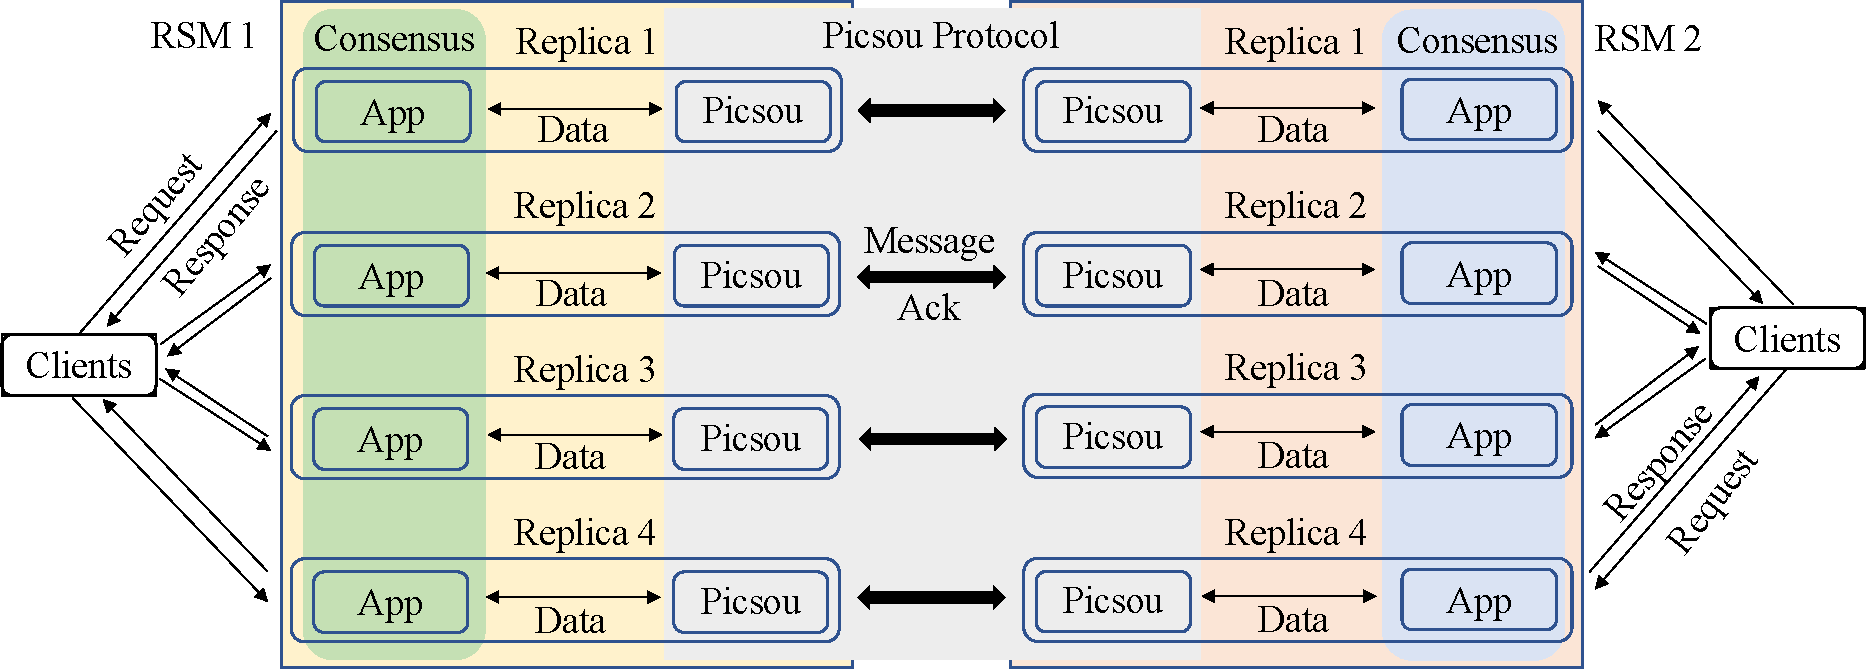
\includegraphics[width=0.85\columnwidth]{end-flow.pdf}
    %\vspace{-2mm}
    \caption{An illustration of \CCC{} primitive between two \RSM{s}, which employ some consensus protocol to manage their states and
    adopt \Scrooge{} for exchanging messages.}
    \label{fig:end-flow}
\end{figure}

\par \textbf{Overview.}  \Scrooge{}'s protocol logic can be  divided into the following logical steps, which we illustrate in Figure~\ref{fig:end-flow}.
\par (1) \textit{Consensus}:  On either side of \Scrooge{} lies a replicated state machine.  Each \RSM{} receives requests from clients and runs a consensus protocol (App) to commit these requests on each \RSM{} replica.
\par (2) \textit{Invoking \Scrooge{}}: Each replica forwards the committed request to the co-located \Scrooge{} library.
\par (3) \textit{Transmitting a message}: \Scrooge{} sends the message on behalf of the sending \RSM{}. In line with our stated efficiency goals, \Scrooge{} ensures that, in the absence of failures and during periods of synchrony, a \textit{single sender} forwards each request to a \textit{single replica} in the receiving \RSM{}. To minimize the risk of repeated failures caused by a faulty sender or receiver, \Scrooge{} carefully {\em rotates} sender-receiver pairs. In doing so, it ensures that every sender will eventually communicate with a correct receiver and vice-versa.
\par (4) \textit{Detecting successful or failed sends:} 
 \Scrooge{} must quickly determine whether a message has definitely been received (and can thus be garbage collected) or has definitely been dropped or delayed. 
Failure detection must be accurate to prevent failed nodes from causing spurious re-transmissions. The key challenge is disseminating this knowledge to all replicas when \Scrooge{} intentionally only sends messages pairwise for efficiency. To this effect, \Scrooge{} adapts TCP's cumulative acknowledgement approach to detect when messages have been received or dropped, even as malicious replicas can lie. These acknowledgements are piggy-backed on incoming messages, thus minimizing overhead. 
\par (5) \textit{Retransmissions}. When the protocol detects that a message has definitely been dropped, \Scrooge{} intelligently chooses the node responsible for resending the message. This is done without any communication across nodes. Unfortunately, without care, Byzantine nodes can selectively drop messages such that throughput craters. To address this issue, \Scrooge{}  includes (constant size) information about which messages have been lost, allowing the protocol to recover dropped messages in parallel. 
Traditional TCP can eschew this constraint as it assumes failures are rare and considers only point-to-point communication between nodes.


\begin{figure}[t]
    %\vspace{-6mm}
    \centering
    \begin{subfigure}[b]{0.32\columnwidth}
         \centering
         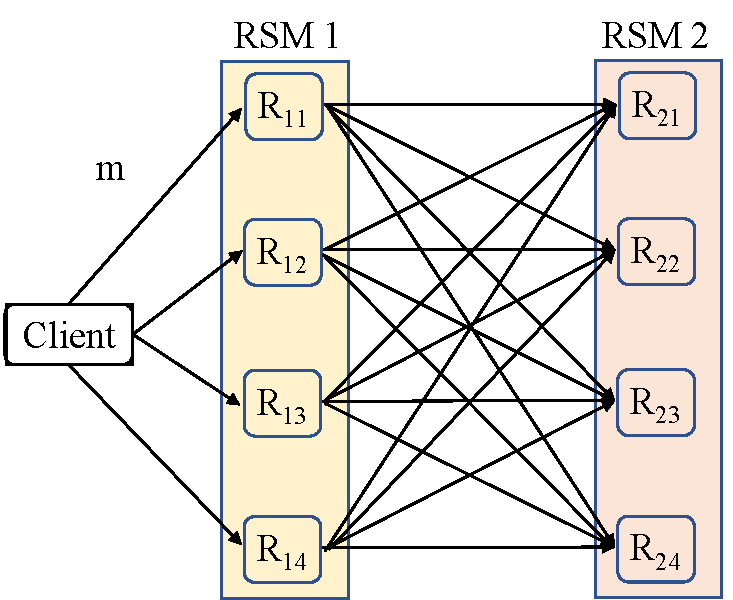
\includegraphics[width=\textwidth]{all-to-all.pdf}
         \caption{All-to-All}
         \label{fig:all-to-all}
     \end{subfigure}%
     \begin{subfigure}[b]{0.32\columnwidth}
         \centering
         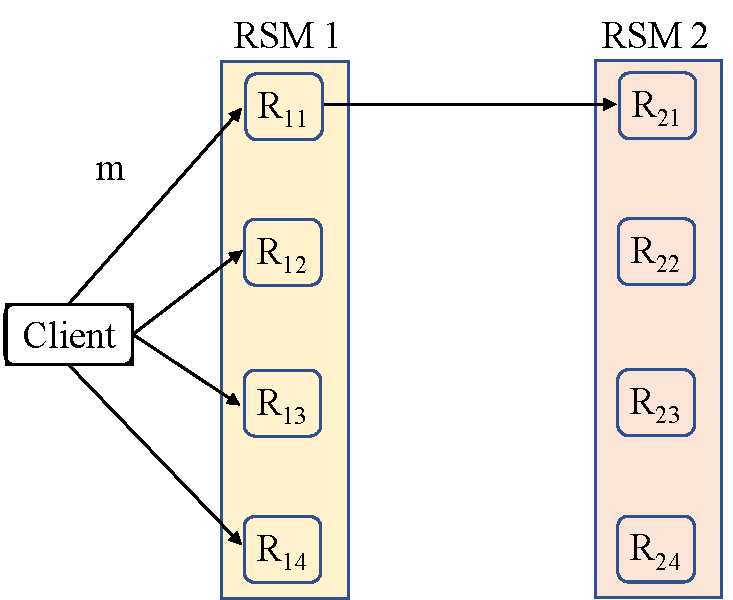
\includegraphics[width=\textwidth]{one-shot.pdf}
         \caption{One-Shot}
         \label{fig:one-to-one}
     \end{subfigure}%
     \begin{subfigure}[b]{0.32\columnwidth}
         \centering
         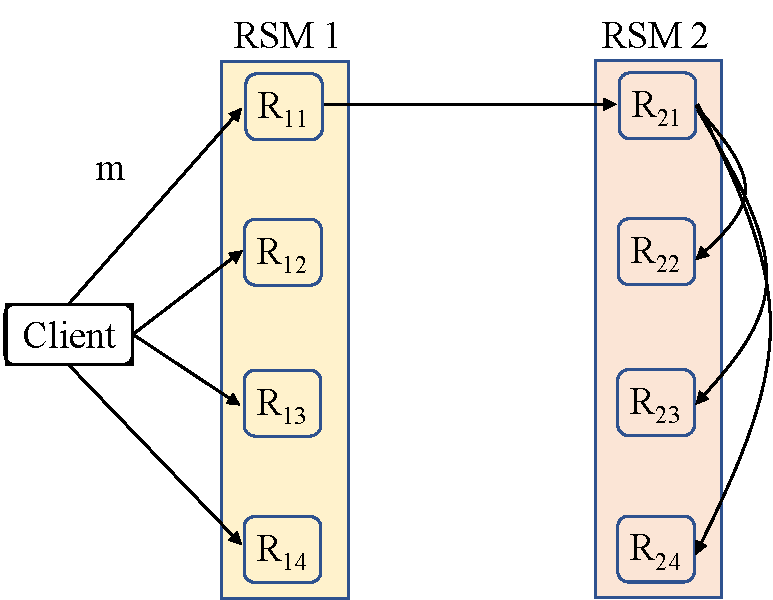
\includegraphics[width=1.05\textwidth]{scrooge.pdf}
         \caption{Picsou}
         \label{fig:scrooge}
     \end{subfigure}
    \caption{Comparison of the number of copies of a message $m$ sent across \RSM{s} by different \CCC{} protocols. 
    Note: One-Shot presents an incomplete design.}
    \label{fig:c3b-protocols}
\end{figure}


\par \textbf{Assumptions.} 
\Scrooge{} assumes knowledge of the current number of replicas in each RSM, failure thresholds, and stake distribution in the system (where applicable). \Scrooge{} further assumes that each request transmitted through \Scrooge{} is of the form $\SignMessage{m, \Seqn}{\Qusign{s}}$, 
where $m$ is a request committed at sequence number $\Seqn$ by a quorum of replicas in \RSM{} $\SMR{s}$. Each protocol sets a specific threshold $t$ above which the request has acquired sufficiently many signatures
$\Qusign{s}$ to be deemed committed. We further assume that all committed requests have contiguous sequence numbers.
\par \textbf{Correctness} We defer a full description of correctness and proofs to our submitted supplemental material.

\section{Protocol Design}

In this section, we describe the details of each logical step: transmitting a message, detecting successful/failed sends, and retransmissions. For simplicity, we ignore stake before revisiting our protocol when nodes have different shares (\S\ref{s:stake}). 
For clarity of exposition, while \Scrooge{} is bidirectional with RSMs acting as both the sender and the receiver, we describe the protocol as consisting of a sender RSM and a receiver RSM. In reality, the protocol is mirrored.

We start by describing \Scrooge{}'s behaviour in the common-case (\S\ref{ss:failurefree}) before considering failures (\S\ref{ss:failures}). 



\begin{figure}[t]
    %\vspace{-6mm}
    \centering
    \begin{subfigure}[t]{0.494\columnwidth}
         \centering
         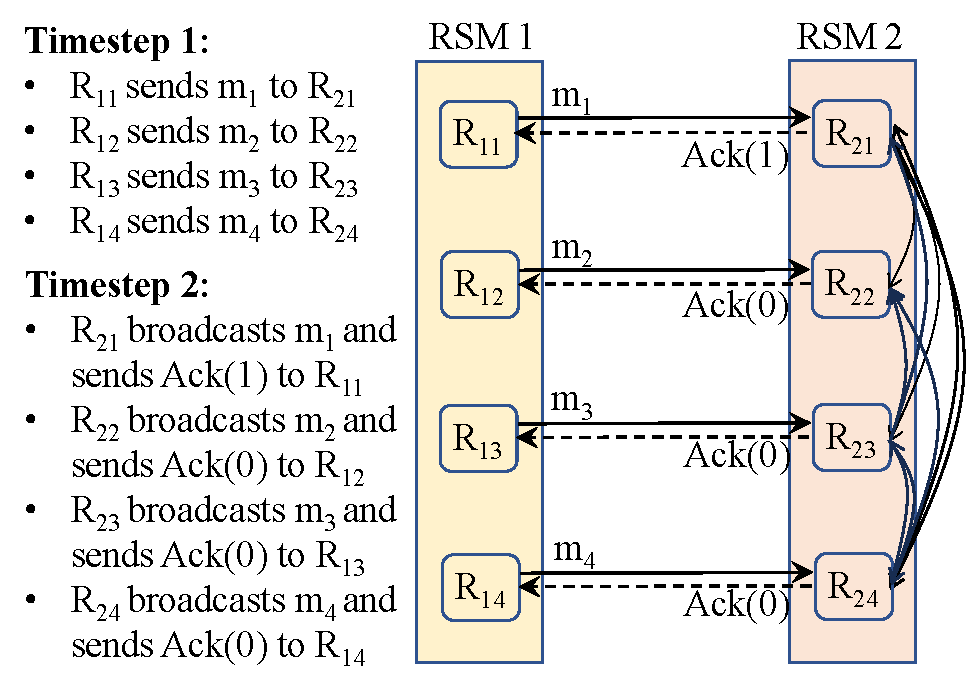
\includegraphics[width=\columnwidth]{acking-p1.pdf}
         %\caption{First set.}
         \label{sfig:first}
     \end{subfigure}
     \begin{subfigure}[t]{0.494\columnwidth}
         \centering
         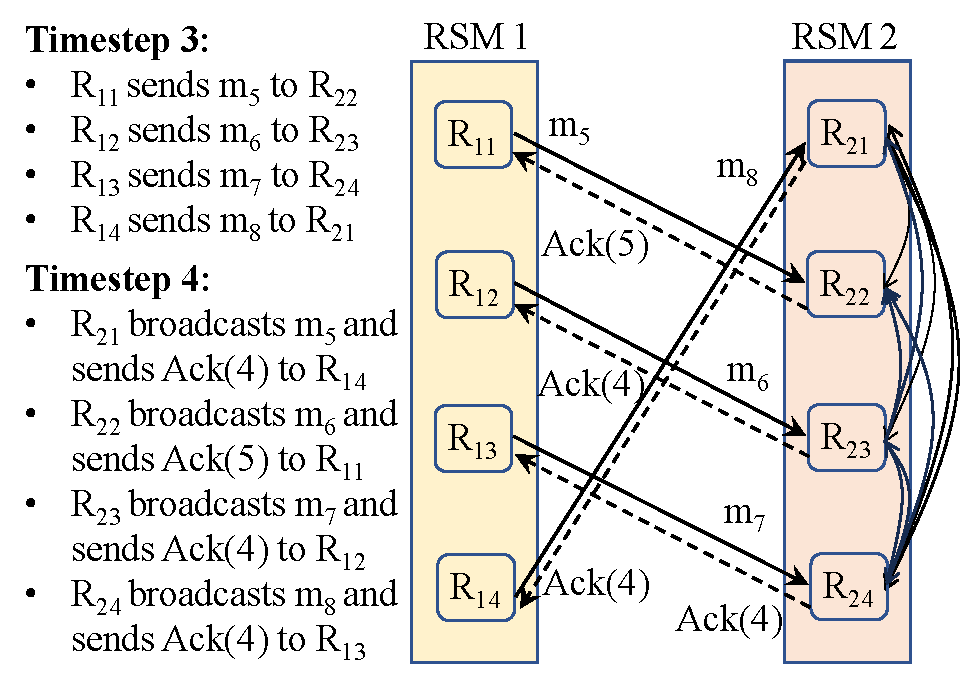
\includegraphics[width=\columnwidth]{acking-p2.pdf}
         %\caption{Second set.}
         \label{sfig:second}
     \end{subfigure}%
    \caption
    {Example failure-free run in \Scrooge{}}
    %This figure illustrates how sender \RSM{} (\RSM{} $1$) forwards messages to receiver \RSM{} (\RSM{} $2$) using \Scrooge{} protocol.
    %Assume the sequence number for messages starts from $1$. 
    %Each \RSM{} $1$ replica sends (round robin) its designated message to a specific replica of \RSM{} $2$. 
    %In turn, it receive a cumulative acknowledgment.
    \label{fig:round-robin}
\end{figure}


\subsection{Failure-free behaviour}
\label{ss:failurefree}

\par \textbf{Sending a message.} \Scrooge{}'s send logic has three goals: 1) minimize the number of nodes sending the same message, 
2) maximize the chances that a message will be successfully transmitted quickly, 
and 3) asynchronously disseminate any knowledge of received messages to all other nodes. 
\Scrooge{} achieves these goals
by partitioning, round-robin, the set of requests to send across all replicas in the sending \RSM, 
and rotating receiver nodes  every round.

By the definition of an \RSM{}, each replica contains a log of committed requests. 
\Scrooge{} evenly partitions the task of transmitting a committed message across all replicas such that each message is sent by a single node: the $l$-th \Scrooge{} node sends messages with sequence number $(\Seqn \bmod \n{s} \equiv l)$. 
Each replica rotates its choice of receiver on every send: if $\n{r}$ is the total number of receivers in the receiver \RSM{}, 
and $j$ is the identifier of the previous recipient, then the $l$-th sender will send to receiver replica $(j+1) \bmod \n{r}$. 
%\rfr{We could also just say node $j$ would send $\Seqn$ to $j+\lfloor\frac{\Seqn}{\n{s}}\rfloor \bmod \n{r}$}.

Rotating sender-receiver pairs in this way guarantees that every pair of replicas will eventually exchange messages and ensures that (1) information about the state of each node is propagated to every other node in the system, and (2) no sender is continuously sending to a faulty replica (or vice-versa). This process is also essential to bounding the number of re-transmissions needed in the presence of failures (more detail in \S\ref{ss:failures}). As is standard in TCP, we allow senders to transmit a window of messages in parallel.
%
%\begin{figure}[h]
%    \begin{myprotocol}
%        \INITIAL{Initialization:}{\newline
%	{%\color{orange}
%	// Let $\MAck{}$ be the list of received messages sorted by sequence number.
%	}}
%	\vspace{1mm}
%
%        \TITLE{Sender-role}{at the $j$-th \Scrooge{} instance at replica $j$}
%        \IF{Message $m$ with sequence $\Seqn$ is such that $k \bmod j = 0$}
%            \IF{$i$ is the identifier of previous receiver replica of receiver \RSM{} $\SMR{r}$}
%                \STATE $rid$ $:=$ $(i+1) \bmod \n{r}$
%                \STATE Send $\SignMessage{m, \Seqn}{\Qusign{s}}$ to receiver with identifier $rid$.
%                \STATE $\{m', p \} :=$ Message with highest sequence $p$ such that $\MAck{}$ has a message for each sequence number $\le p$.
%                \STATE Piggyback $\Ack{p}$ with message $\SignMessage{m, \Seqn}{\Qusign{s}}$.
%            \ENDIF
%        \ENDIF
%        \SPACE
%
%        \TITLE{Receiver-role}{at the $i$-th \Scrooge{} instance at replica $i$}
%        \EVENT{Received message $\SignMessage{m, \Seqn}{\Qusign{s}}$ from $j$-th replica of \RSM{} $\SMR{s}$}
%            \STATE Broadcast $\SignMessage{m, \Seqn}{\Qusign{s}}$ in its \RSM{} $\SMR{r}$.
%            \STATE Add $\{m, \Seqn \}$ to list $\MAck{}$.
%        \ENDEVENT
%    \end{myprotocol}
%    \caption{\Scrooge{} code running at the sender and receiver replicas.\nc{We need to be consistent with pseudocode and text}}
%    \label{alg:scrooge-no-fail}
%\end{figure}
%%


\par \textbf{} Upon receiving a message, the $j$-th replica $\Replica{r}{j}$ checks that the message $\SignMessage{m, \Seqn}{\Qusign{s}}$ is valid (the message has provably been committed by the sender \RSM{}) and if so, broadcasts it to the other nodes in its \RSM{}.  In the failure-free case,
\Scrooge{} thus sends a total of $\n{r}$ messages. This is in line with the theoretical minimum of all \CCC{} protocols.

\begin{figure}[t]
    %\vspace{-6mm}
    \centering
    \begin{subfigure}[b]{0.32\columnwidth}
         \centering
         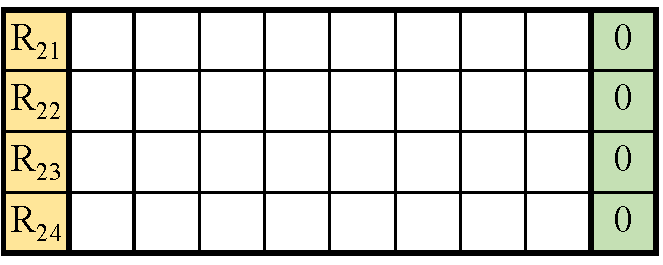
\includegraphics[width=\textwidth]{cack1.pdf}
         \caption{Initial}
         \label{sfig:initial}
     \end{subfigure}
     \begin{subfigure}[b]{0.32\columnwidth}
         \centering
         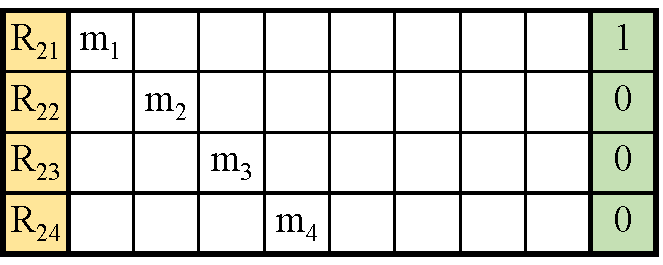
\includegraphics[width=\textwidth]{cack2.pdf}
         \caption{Timestep 1}
         \label{sfig:first-set}
     \end{subfigure}
     \begin{subfigure}[b]{0.32\columnwidth}
         \centering
         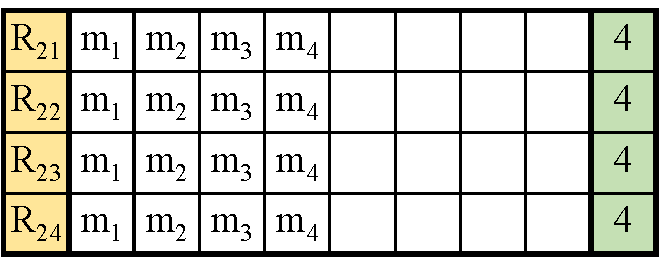
\includegraphics[width=\textwidth]{cack3.pdf}
         \caption{Timestep 2}
         \label{sfig:first-broadcast}
     \end{subfigure}
     \begin{subfigure}[b]{0.32\columnwidth}
         \centering
         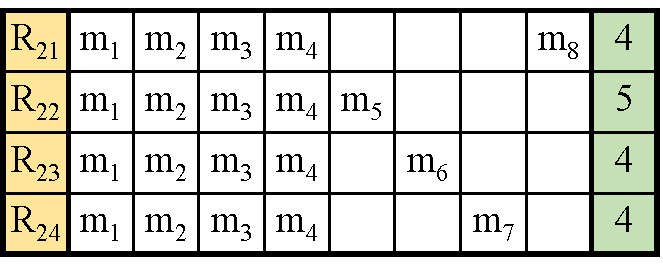
\includegraphics[width=\textwidth]{cack4.pdf}
         \caption{Timestep 3}
         \label{sfig:second-set}
     \end{subfigure}
     \begin{subfigure}[b]{0.32\columnwidth}
         \centering
         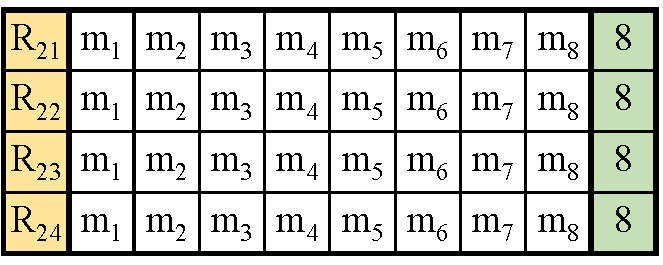
\includegraphics[width=\textwidth]{cack5.pdf}
         \caption{Timestep 4}
         \label{sfig:second-broadcast}
     \end{subfigure}
    \caption{Receiver's view of events in Figure~\ref{fig:round-robin}.}
    \label{fig:ack-counter}
\end{figure}

We illustrate \Scrooge's logic in Figure~\ref{fig:round-robin}.
Note that, in each time-step, we assume that a replica completes all the relevant tasks in parallel. Consider a system
with $\n{r} = 4$ replicas ($\uf{}= \rf{} = 1$).
In Timestep 1, replicas $\Replica{1}{1}$, $\Replica{1}{2}$, and $\Replica{1}{3}$
of $\RSM{}_1$ send messages
 $m_1$, $m_2$, and $m_3$ respectively to receivers $\Replica{2}{1}$, $\Replica{2}{2}$, and $\Replica{2}{3}$. 
In Timestep 2 \nc{1?}, these replicas internally broadcast these messages to the other nodes
in their \RSM{}.
Concurrently, $\Replica{2}{1}$, $\Replica{2}{2}$, and $\Replica{2}{3}$ acknowledge receipt of these messages and send $\Ack{1}$, $\Ack{0}$, and $\Ack{0}$ to senders 
$\Replica{1}{1}$, $\Replica{1}{2}$, and $\Replica{1}{3}$.
We discuss acknowledgements later in the section.
In Timestep 3, $\Replica{1}{1}$, $\Replica{1}{2}$, and $\Replica{1}{3}$ rotate receivers and
send messages $m_5$, $m_6$, and $m_7$ to $\Replica{2}{2}$, $\Replica{2}{3}$, and $\Replica{2}{4}$.
In Timestep 4, these replicas once again broadcast the received messages to the other nodes in their \RSM{}.
Simultaneously, $\Replica{2}{1}$, $\Replica{2}{2}$, and $\Replica{2}{3}$ send $\Ack{4}$, $\Ack{5}$, and $\Ack{4}$ to senders 
$\Replica{1}{4}$, $\Replica{1}{1}$, and $\Replica{1}{2}$, respectively. 
\par \textbf{Detecting successful sends.} To guarantee correctness, all committed messages must eventually be received by an honest node in the receiving \RSM{}. The sending \RSM{} must thus detect when its message has \textit{definitely} been received by an honest node. Specifically, all honest nodes in the sending \RSM{} (not just the sender) must learn that a message was successfully delivered. This is necessary to preclude honest nodes from unnecessarily resending messages.

There are three primary challenges: (1) malicious nodes may lie about the set of messages received, (2) for efficiency, \Scrooge{} should not require nodes within an \RSM{} to exchange information beyond the necessary message broadcast, and (3) any additional metadata should be small. \Scrooge{} realizes these goals through \textit{cumulative quorum acknowledgements} (or \quack{}s). A cumulative quorum acknowledgement with value $\Seqn$ proves to the sending \RSM{} that all messages with sequence number up to $\Seqn$ have been received by at least one honest replica. 

More specifically, each replica, upon receiving a message with sequence number $\Seqn$, inserts it into a sorted list containing all previously received messages. The replica does not, however, \textit{selectively} acknowledge $m_k$. Instead, it identifies the highest message $m_p$ in the list for which all messages with a smaller sequence number have been received. The replica crafts an acknowledgement $\Ack{p}$ that cumulatively acknowledges receipt of messages $0$ to $p$. \Scrooge{} takes advantage of the full-duplex nature of the protocol to piggy-back these acknowledgements onto the messages that the receiving \RSM{} is itself sending to the sending \RSM{}. If no such message exists, the \RSM{} sends a no-op.
%Note \msg{Not sure if this sentence will be clear to a reader. At present it seems like some senders may not receive cumulative acknowledgment?}\mnc{Fair point. Happy to remove}
%that this implies that the acknowledgement for message $p$ may not be sent back to the initial sender of $p$, but to another replica in the sending \RSM{}.

On the sender side, each replica eventually receives messages and acknowledgements from all $\n{r}$ receiving replicas, thanks to \Scrooge{}'s round-robin strategy.  Each replica maintains an $\n{r}$ sized array that summarizes the highest acknowledgement received from each replica of the receiving \RSM{}. There exists a \quack{} for message $m_p$ (we say message $m_p$ has been \quack{}ed) if at least $\uf{r} + 1$ array entries have a value greater or equal to $p$, which indicates that $\uf{r}+1$ replicas have acknowledged receipts of all messages up to $p$. As there are only $\uf{r}$ failed replicas, one of these replicas must be honest. We thus have the guarantee that this correct replica will broadcast the message to all other remaining honest participants. Note that \Scrooge{} additionally uses MACs when configured to handle Byzantine failures ($\rf{}>0$)
%\begin{figure}[h]
%    \begin{myprotocol}
%        \INITIAL{Initialization:}{\newline
%	{%\color{orange}
%	// Let $\QuArr{}$ be the array of $\n{r}$ size.\newline
%        // Let $\highest$ be the largest \quack{ed} value 
%	}}
%	\vspace{1mm}
%
%        \EVENT{Received $\Ack{p}$ from $i$-th replica of \RSM{} $\SMR{r}$}
%            \STATE Set $\QuArr{i} := p$.
%            \WHILE{true}
%                \IF{$\f{r} + 1$ entries of $\QuArr{}$ have value $\ge \highest + 1$}
%                    \STATE Garbage collect message with sequence number $\highest$
%                    \STATE $\highest ++$
%                \ELSE
%                    \STATE break;
%                \ENDIF
%            \ENDWHILE
%        \ENDEVENT
%    \end{myprotocol}
%    \caption{Cumulative quorum acknowledgments at sender.}
%    \label{alg:scrooge-no-fail}
%\end{figure}
%

\par \textbf{Example.} To illustrate our message \quack{}ing logic, 
we continue with our example in Figure~\ref{fig:round-robin}.
Figures~\ref{fig:ack-counter} and ~\ref{fig:quack-counter} describe the protocol logic for, respectively, the receiver RSM and the sender RSM.  
Each row in Figure~\ref{fig:ack-counter} summarizes the sorted list of messages received at each replica, 
with the last column denoting the highest cumulative acknowledgment for this node.
Initially, all lists are empty and cumulative acknowledgment values are all set to $0$ (\ref{sfig:initial}). 
At Timestep 1, 
receivers $\Replica{2}{1}$, $\Replica{2}{2}$, and $\Replica{2}{3}$ (\ref{sfig:first-set}) store messages $m_1$, $m_2$ and $m_3$.
$R_{21}$'s cumulative acknowledge counter thus increases to 1, while others stay at 0 as they are still missing $m_1$. 
$\Replica{2}{1}$, $\Replica{2}{2}$, and $\Replica{2}{3}$ thus send $\Ack{1}$, $\Ack{0}$ and $\Ack{0}$ to the sender RSM.
At Timestep 2, each receiver, thanks to the internal broadcast mechanism, receives all three messages. All cumulative acknowledgement counters thus go to $4$ (\ref{sfig:first-broadcast}). By Timestep 3, receivers $\Replica{2}{1}$, $\Replica{2}{2}$, and $\Replica{2}{3}$ have all received $m_8$, $m_5$ and $m_6$.
$\Replica{2}{2}$ has received messages $m_1$ to $m_5$, and thus updates its cumulative acknowledgement to $5$. In contrast,
through $\Replica{2}{1}$ and $\Replica{2}{3}$ have received messages $m_8$ and $m_6$ respectively, they are missing $m_5$ and thus cannot
yet update their cumulative acknowledgement counter. Each replica sends $\Ack{4}$, $\Ack{5}$ and $\Ack{4}$ back to the sending RSM.
Finally, at Timestamp 4, the internal broadcast mechanism disseminates all these messages; each replica can update its cumulative acknowledgement to 8, and send $\Ack{8}$ back to the initiating RSM. 

Consider instead the protocol logic at the sender-side (Figure~\ref{fig:quack-counter}), which processes these cumulative acknowledgements and determine when a \quack{}
has formed. Each replica maintains an array summarising how many acknowledgements have been received for each message. A message is \quack{}ed at a replica if this replica receives $\uf{}+1=2$ acknowledgements for $m$.
 Initially, \quack{} counters at each replicas are empty (\ref{sfig:init-ack}). At Timestamp $2$, $\Replica{1}{1}$
(\ref{sfig:first-ack})'s records that it has received an acknowledgement for $m_1$  ($\Ack{1}$) from $\Replica{2}{1}$. 
At Timestamp 4, (\ref{sfig:second-ack}), $\Replica{1}{1}$ receives $\Ack{5}$ from $\Replica{2}{2}$. It updates its local array
to reflect that it now has received two acknowledgements for $m_1$, and \quack{}s $m_1$. It further reflects receipt of acknowledgements
for $m_2$, $m_3$, $m_4$, and $m_5$. $\Replica{1}{2}$ and $\Replica{1}{3}$ similarly indicate that they have received acks for $m_1$, $m_2$, $m_3$, and $m_4$
as they both received $\Ack{4}$. 

\begin{figure}[t]
    %\vspace{-6mm}
    \centering
    \begin{subfigure}[b]{0.32\columnwidth}
         \centering
         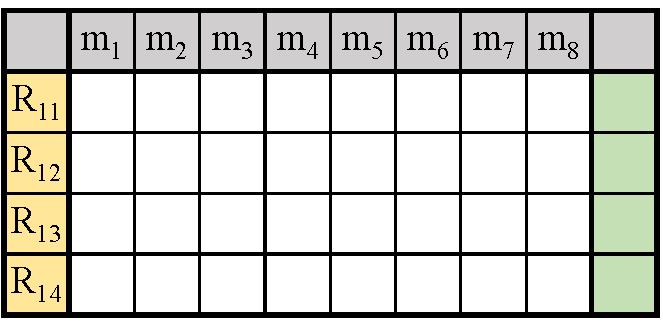
\includegraphics[width=\textwidth]{quack1.pdf}
         \caption{Initial}
         \label{sfig:init-ack}
     \end{subfigure}
     \begin{subfigure}[b]{0.32\columnwidth}
         \centering
         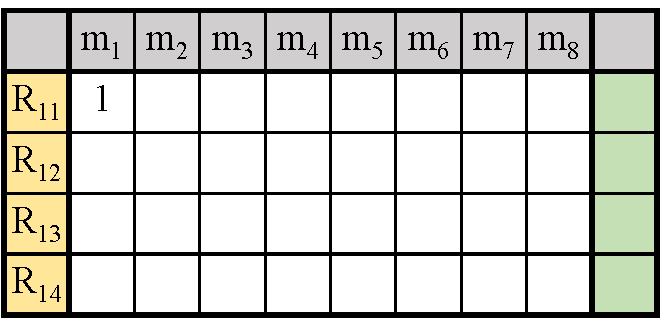
\includegraphics[width=\textwidth]{quack2.pdf}
         \caption{Timestep 2}
         \label{sfig:first-ack}
     \end{subfigure}
     \begin{subfigure}[b]{0.32\columnwidth}
         \centering
         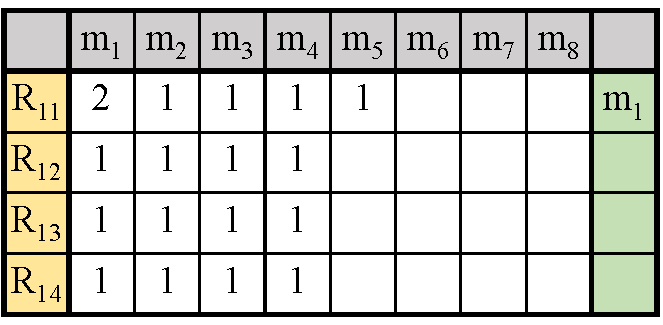
\includegraphics[width=\textwidth]{quack3.pdf}
         \caption{Timestep 4}
         \label{sfig:second-ack}
     \end{subfigure}
    \caption{Sender's view of events in Figure~\ref{fig:round-robin}.}
    \label{fig:quack-counter}
\end{figure}

\par \textbf{Summary} The joint techniques of full-duplex communication, cumulative acking, and rotation of sender/receiver pairs allows \Scrooge{} to ensure that all replicas in an \RSM{} will eventually learn that all committed requests have been reliably received by the receiving \RSM{}. In line with its efficiency goals, the protocol achieves this with only two additional counters, and with no additional communication between the replicas of an \RSM{} beyond the necessary broadcast.  The use of \quack{}s is key to \Scrooge{}'s generality: they require no synchrony assumptions and simply require that the sending \RSM{} know the failure threshold of the receiving \RSM{}. 

\subsection{Handling Failures}
\label{ss:failures}
Crashed replicas can fail to complete a send or broadcast; byzantine replicas can either intentionally drop messages (whether when sending or receiving) or lie in their acknowledgements. They can, for instance, spuriously advance their ack, thus potentially causing honest senders to believe that their message has been received, or, on the contrary, send an intentionally low ack, causing honest replicas to spuriously resend messages.  \Scrooge{} must effectively handle these failures without sacrificing correctness or performance. To this effect,  \Scrooge{} must quickly and reliably detect \textit{when} a message has \textit{definitely} been dropped and quickly retransmit it. The system must do so without any additional intra or inter-\RSM{} communication beyond resending the message itself. 

\par \textbf{Detecting definitely failed sends.} The protocol once again leverages \quack{}s.   Recall that all sender replicas eventually obtain a \quack{} for every message that has \textit{definitely} been delivered. One can instead leverage duplicate 
\quack{}s to determine when an honest replica has \textit{definitely not} received a specific message. 
In more detail, let us assume that a \quack{} for message $m_k$ has formed at $\Replica{s}{l}$. 
This \quack{} indicates that at least $\uf{} + 1$ (at least one honest) replicas have received every message up to message $m$ with sequence number $k$.  
If one of these replicas sends a duplicate acknowledgement $\Ack{k}$ for $m$, one can conclude that this replica claims to not have received message at sequence number $k + 1$. Once a duplicate \quack{} forms for the $k$-th message at replica $\Replica{s}{l}$,  $\Replica{s}{l}$ can reliably infer that $(k+1)$-th message has been lost or delayed as an honest replica is complaining about the missing message. All other honest replicas of the sending \RSM{} $\SMR{s}$ will eventually receive a duplicate \quack{} and thus detect the failed exchange.
The use of the Upright failure model, which distinguishes malicious failures $\rf{}$ from all other failures, allows us to reduce the size of the duplicate \quack{}: while the initial \quack{} is of size    $\uf{} + 1$, duplicate \quack{}s must be of size $\rf{} + 1$ as they must be large enough to preclude actively malicious nodes from triggering spurious resends. In contrast, a faulty node (one that will eventually crash) sending a duplicate acknowledge still signals the existence of a faulty sender/receiver or dropped message. As such, in a system with only crash failures (when $\rf{}=0$), a single duplicate \Ack{} is sufficient to trigger a message resend.

\par \textbf{Retransmitting the dropped message.} Upon detecting a failed send, the message must be quickly retransmitted. Just as a single replica was responsible for sending the initial message, \Scrooge{} ensures that a single replica is "elected" as the retransmistter. It does so \textit{without} requiring additional communication between replicas. The protocol logic hinges on three observations: 1) all correct replicas know about all the messages that must be transmitted (by definition of an \RSM{}) and know who initially sent the message, 2) all correct replicas eventually learn about which messages have been \quack{}ed,
3) the number of repeated \quack{}s indicate the number of failed retransmissions. 
\Scrooge{} uses this information to compute the ID of the retransmitter as: $sender_{new} = sender_{original} + (\#_{retransmit} \mod \n{sender})$.  Each honest replica computes this function, and retransmits the message if its ID matches $sender_{new}$.  Each retransmission round thus has a single sender.


\begin{figure}[t]
    %\vspace{-6mm}
    \centering
    \begin{subfigure}[b]{0.3\columnwidth}
         \centering
         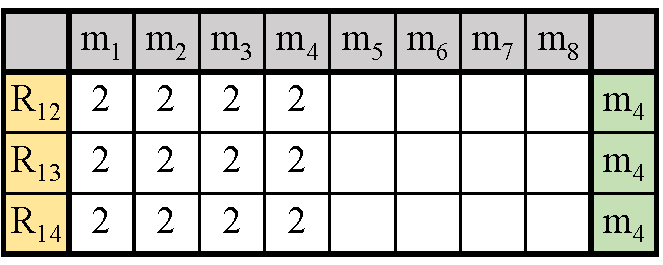
\includegraphics[width=\textwidth]{fail-quack1.pdf}
         \caption{Timestep 6}
         \label{ssfig:init-ack}
     \end{subfigure}
     \begin{subfigure}[b]{0.3\columnwidth}
         \centering
         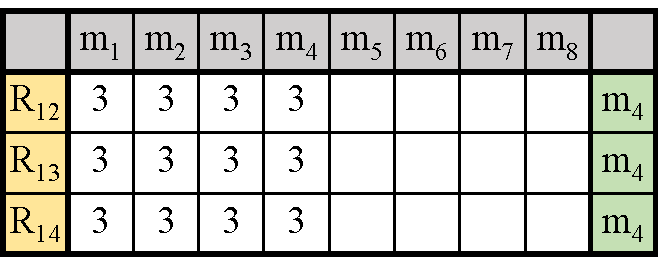
\includegraphics[width=\textwidth]{fail-quack2.pdf}
         \caption{Timestep 8}
         \label{ssfig:first-ack}
     \end{subfigure}
     \begin{subfigure}[b]{0.3\columnwidth}
         \centering
         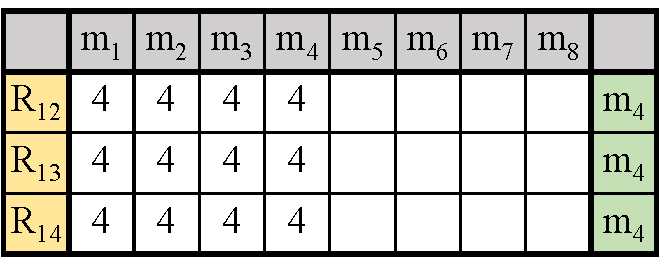
\includegraphics[width=\textwidth]{fail-quack3.pdf}
         \caption{Timestep 10}
         \label{ssfig:second-ack}
     \end{subfigure}

     \begin{subfigure}[b]{0.3\columnwidth}
         \centering
         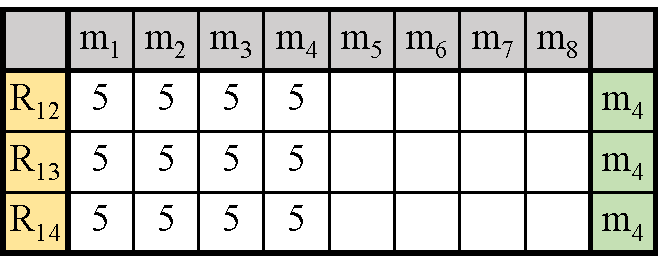
\includegraphics[width=\textwidth]{fail-quack4.pdf}
         \caption{Timestep 12}
         \label{usfig:init-ack}
     \end{subfigure}
     \begin{subfigure}[b]{0.3\columnwidth}
         \centering
         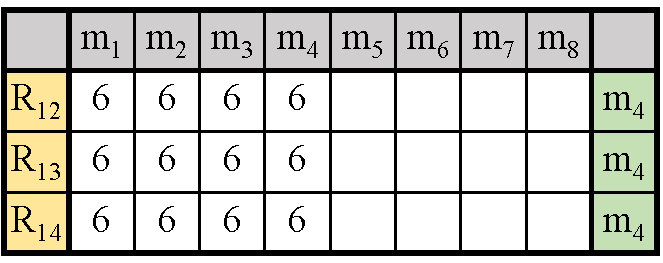
\includegraphics[width=\textwidth]{fail-quack5.pdf}
         \caption{Timestep 14}
         \label{usfig:first-ack}
     \end{subfigure}
     \begin{subfigure}[b]{0.3\columnwidth}
         \centering
         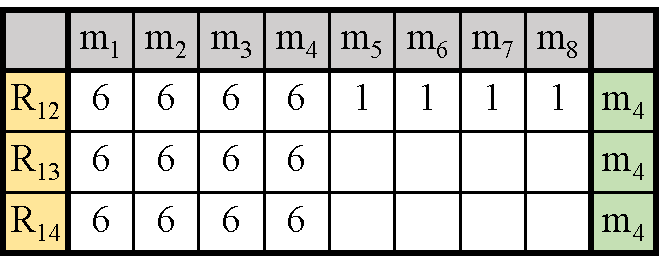
\includegraphics[width=\textwidth]{fail-quack6.pdf}
         \caption{Timestep 16}
         \label{usfig:second-ack}
     \end{subfigure}
    \caption{Sender's view of events if replica $\Replica{1}{1}$ fails after Timestep 2 (does not send any message after $m_1$) in Figure~\ref{fig:round-robin}. }
    \label{fig:fail-quack-counter}
\end{figure}

To illustrate, consider once again our initial example (Figure~\ref{fig:round-robin}), but this time, let us assume that sender replica $\Replica{1}{1}$ fails after sending message $m_1$ but before sending messages $m_5$ and $m_9$. As a result, no receiver receives these messages. In Figure~\ref{fig:fail-quack-counter}, we timestep through this failure scenario. For simplicity of exposition, we assume that senders (except $\Replica{1}{1}$) send new messages in odd timesteps and receive cumulative acknowledgements in even timesteps. 
%
As $\Replica{1}{1}$ fails after sending $m_1$ (at the end of Timestep 4) every other replica of \RSM{1} receives cumulative acknowledgment 
message $\Ack{4}$ for the first time (Figure~\ref{fig:round-robin}).
These senders continue sending remaining messages, so by Timestep 6, all senders
have received  $\Ack{4}$ messages twice (from $\uf{r}+1 =2$ receivers). This allows them to mark messages $m_1$ to $m_4$ as \quack{ed}. 
These receivers cannot acknowledge any message greater than $m_4$ as they are yet to receive $m_5$.
The senders are yet to receive $\Ack{4}$ messages from the remaining replicas (in our case $2$ other replicas).
They receive these acknowledgments during Timesteps 8 and 10. 
At the end of Timestep 10, each sender has received $\Ack{4}$ from each receiver in $\SMR{r}$.
Next, in Timestep 12, each sender will receive its first duplicate $\Ack{4}$ message; 
it has already received an $\Ack{4}$ message from this receiver (during Timestep 4).
By the end of timestep 14, each sender has received at least $\rf{r}+1 =2$ duplicate $\Ack{4}$ messages, which 
informs the senders that message $m_5$ is missing.
As a result, $\Replica{1}{2}$ proceeds to resend $m_5$.


\par \textbf{The pitfalls of sequential recovery.} 
Unlike traditional TCP in which message drops are not adversarial, Byzantine replicas can carefully select which messages to drop. 
For instance,  in a $\n{} = 2\uf{}+ \rf{} +  1$ setup with $\uf{} = \rf{}= 1$, if a malicious actor drops all received messages, every fourth message will need to be resent.
In this setup, \Scrooge{} as currently described unfortunately introduces an artificial throughput bottleneck as the system maintains a single cumulative acknowledgement. A \quack{} conveys information about the \textit{lowest} message that has been dropped by the system, but says nothing about later messages.  This approach is optimal metadata-wise but serializes recovery: if messages $m_i$, $m_{i+4}$, $m_{i+8}$, etc. have all been dropped, 
resending $m_{i+8}$ first requires detecting the failed send of message $m_i$, retransmitting $m_i$, \quack{} $m_i$, before repeating
the same process for $m_{i+4}$. Only then can the failed send of $m_{i+8}$ be handled.


%\nc{Sequential recovery artificially throttles the system to sending a maximum of. Not done here yet. See Suyash's explanation in comments}
%Assume replicas of \RSM{} $\SMR{1}$ and \RSM{} $\SMR{2}$ (in Figure~\ref{fig:round-robin}) are working in
%the following ideal model:
%(1) Each replica of $\SMR{1}$ has an infinite stream of messages to send.
%(2) Instead of sending one message per timestep, each replica of $\SMR{1}$ sends $N$ messages in each timestep, and
%(3) Instead of acknowledging one message per timestep, each replica of $\SMR{2}$ acknowledges $N$ messages in each timestep.
%Consequently, in this model, each replica of $\SMR{1}$ will receive $N$ \quack{s} every timestep.
%So, in one RTT (sending message + receiving cumulative acknowledgments), the sending throughput is $N \times \n{1}$
%($\n{1}$ is the number of replicas in $\SMR{1}$).
%
%Now, assume replica $\Replica{1}{3}$ fails, which results in non-delivery of every third message ($m_3, m_6,...$).
%As each replica receives infinite number of \quack{s} per timestep, it will also receive infinite number of duplicate \quack{s} in that timestep.
%However, \Scrooge{} requires replicas to send duplicate \quack{s} for one missing message at a time.
%For instance, in the timestep, when replicas of $\SMR{1}$ receive \quack{s} for $m_1$ and $m_2$, they will receive
%infinite duplicate \quack{s} for $m_3$.
%So, in the following timestep replicas $\Replica{1}{1}$ and $\Replica{1}{2}$ will resend $m_3$.
%This will result in receiving infinite number of duplicate \quack{s} for $m_6$ in the subsequent timestep.
%Following this pattern, we can conclude that the system throughput is $1 \times \n{1}$ per RTT.
%This illustrates that sequential recovery of dropped messages decreases system throughput by $N\times$.
%
%

\par \textbf{Parallel Cumulative Acknowledgments.} 
To address this issue, we must augment our cumulative acknowledgments with a limited form of selective repeat~\cite{selective-repeat}.
Each receiver sends both a cumulative acknowledgement and bounded size list ($\phi$) of messages that it is missing. The cumulative acknowledgement counter concisely summarises the list of contiguous messages received so far while the $\phi$-list captures any "in-flight" missing messages. Sender replicas can now, concurrently, form \quack{s} for $\phi$ concurrent messages and thus retransmit $\phi$ messages in parallel.  
The maximum size of $\phi$-list is an experiment-specific parameter, which is measured as function of
\Scrooge's steady state network bandwidth and latency for retransmission under failures.
The actual number of elements in a $\phi$-list depends on the number of missing messages at a replica at the time of sending a cumulative acknowledgement.



\par \textbf{Analysis.} 
During periods of synchrony (when messages are not delayed by the network), \Scrooge{} retransmits messages at most $\uf{s} + \uf{r}+ 1$ times. While this limitation is fundamental to all \CCC{} protocols (Theorem 1 in Supplementary Material), the number of resends is still a theoretical concern for latency if the number of failures is large. 
In practice, however, the probability of actually hitting this bound is vanishingly small. In fact, assuming a fixed ratio of Byzantine nodes in the system, each with a random identifier, after only 8 retries, the probability that a message was successfully delivered is already 99.9\%, independently of RSM size.

\begin{theorem}
 Given a sending \RSM{} with $\n{s}= \alp{s} \times \uf{s} + 1$ replicas and 
receiving \RSM{} with $\n{r}= \alp{r} \times \uf{r} + 1$ replicas, where $\alp{s}, \alp{r} > 1$ are the replication factors of the \RSM{s},
\Scrooge{} needs to resend a message at most $72$ times to guarantee a $10^{-9}$ failure probability, irrespective of the number of nodes and failures.
\end{theorem}
\begin{proof}
The maximum number of faulty pairs (either the receiver or the sender is faulty) in this system of two \RSM{s} is:
\begin{equation}
Faulty = \uf{s} \times \n{r} + \uf{r} \times \n{s} - \uf{s} \times \uf{r}   
\end{equation}
By assumption, we have $\uf{s} = \frac{\n{s}-1}{\alp{s}}$ and $\uf{r} = \frac{\n{r}-1}{\alp{r}}$.
We get:
\begin{equation}\label{eq:2}
\begin{split}
Faulty  & = \frac{\n{s} \times \n{r}}{\alp{s}} + \frac{\n{r} \times \n{s}}{\alp{r}} - \frac{\n{s} \times \n{r}}{\alp{s} \times \alp{r}} \\
        & - \frac{\n{r}}{\alp{s}} - \frac{\n{s}}{\alp{r}} + \frac{\n{s} + \n{r}}{\alp{s} \times \alp{r}} - \frac{1}{\alp{s} \times \alp{r}}
\end{split}
\end{equation}
Given that $\alp{s}, \alp{r} > 1$, which is typical for any fault-tolerant \RSM{}, the following holds. 
\begin{equation}\label{eq:3}
    - \frac{\n{r}}{\alp{s}} - \frac{\n{s}}{\alp{r}} + \frac{\n{s} + \n{r}}{\alp{s} \times \alp{r}} - \frac{1}{\alp{s} \times \alp{r}} < 0
\end{equation}
From Equations~\ref{eq:2} and~\ref{eq:3}, we have:
\begin{equation}\label{eq:4}
Faulty  < \frac{\n{s} \times \n{r}}{\alp{s}} + \frac{\n{r} \times \n{s}}{\alp{r}} - \frac{\n{s} \times \n{r}}{\alp{s} \times \alp{r}}
\end{equation}
\begin{equation}\label{eq:5}
\begin{split}
\frac{Faulty}{\n{s} \times \n{r}}   & < \frac{1}{\alp{s}} + \frac{1}{\alp{r}} - \frac{1}{\alp{s} \times \alp{r}} \\
                                    & = \frac{\alp{r} + \alp{s} - 1}{\alp{s} \times \alp{r}}
\end{split}
\end{equation}
 $\frac{\alp{r} + \alp{s} - 1}{\alp{s} \times \alp{r}} <= \frac{3}{4}$ for $a_s,a_r>=2$. When substituted in Equation~\ref{eq:5} gives $\frac{Faulty}{\n{s} \times \n{r}} <= \frac{3}{4}$.
 $\frac{Faulty}{\n{s} \times \n{r}}$ is also the probability of selecting a faulty pair ($p_{fail}$).
So, the probability of selecting $q$ faulty pairs for resends is:
\begin{equation}
 (\frac{Faulty}{\n{s} \times \n{r}})^q  <= (\frac{3}{4})^q
\end{equation}
Solving for $q$ gives $q = \lceil \log_{\frac{3}{4}}{p_{fail}} \rceil$.
For $p_{fail} = 1 \times 10^{-9}$, we need at most $q = 72$ resends.
\end{proof}

\subsection{Garbage Collection}
\label{ss:garbage}

Garbage collecting messages in \Scrooge{} is, in theory, straightforward. The sending \RSM{}, upon receiving a \quack{} for $m$ should be able to garbage collect $m$ as quacking a message provides the guarantee that it has already been received by an honest replica.  This naive implementation of garbage collection is unfortunately not quite sufficient and can lead to scenarios in which \Scrooge{} grounds to a halt. Consider, for instance, an execution in which  sender $\Replica{s}{l}$ sends a message $m_\Seqn$ (at sequence number $\Seqn$) 
to replica $\Replica{r}{j}$ of \RSM{} $\SMR{r}$. Now, consider the case in which
$\Replica{r}{j}$ is byzantine and broadcasts $m_\Seqn$ to precisely $\uf{r}+1$ replicas, $\uf{r}$ of which are faulty. These replicas reply to the sender RSM that $m$ has been successfully received, allowing for a \quack{} to form at the sender, and for message $m$ to be garbage collected. Unfortunately, if these $\uf{r}$ replicas then stop participating in the protocol, no \quack{} will ever form for any message with sequence number greater than $\Seqn$ (only one honest replica has seen $m$). Instead, the sending RSM will receive repeated duplicate acknowledgements for $m$, a message which it has already garbage collected!

We must consequently modify the garbage collection algorithm slightly. If a sending replica ever receives a duplicate \quack{} for message $m_{\Seqn'}$ where $\Seqn'<\Seqn$ \textit{after} having quacked and garbage collected message $m_\Seqn$, it includes, as additional metadata, the sequence number $\Seqn$ of its highest quacked message. This information conveys to the receiving RSM that all messages up until $\Seqn$ (included) have been received by \textit{some} honest node in the receiving RSM, but not necessarily the same one. Replicas in the receiving RSM, after having received $\rf{s}+1$ such messages (ensuring that at least one honest node is in the set), can then either (1) advance their cumulative acknowledgment counter to $\Seqn$ and mark message $m$ as received, or (2) ask replicas in its \RSM{} if they have access to $m$. We intentionally offer both strategies as \CCC{} only requires that \textit{some} honest replica receive the message, not all honest replicas.

%\Scrooge{} expects the replicas of the sending \RSM{} $\SMR{s}$ to store a message $m$ until they receive acknowledgments
%for $m$ from $\uf{r}+1$ replicas of the receiving \RSM{} $\SMR{r}$.
%Post receiving $\uf{r}+1$ acknowledgments (\quack{}) for $m$, a replica $\Replica{s}{l}$ of \RSM{} $\SMR{s}$ can delete $m$.
%This deletion is necessary to ensure that $\Replica{s}{l}$ requires a fixed-size memory to run \Scrooge{}.
%Unfortunately, garbage collecting a message $m$ after receiving a \quack{} for $m$ 
%can often lead to a case where a majority of correct receivers (we refer to them as receivers in the dark) never receive $m$. 
%For example, when a sender $\Replica{s}{l}$ forms a \quack{} for message $m$ with sequence number $\Seqn$, 
%even if, in the future, it receives a duplicate \quack{} for the message with sequence number $m-1$, 
%it will ignore this duplicate \quack{} as $\Replica{s}{l}$ knows that at least one honest receiver has access to $m$.
%However, receivers in the dark do not know that senders have a \quack{} for $m$; 
%from the perspective of receivers in the dark, $m$ is missing and they expect some sender in \RSM{} $\SMR{s}$ to resend $m$.
%
%On extrapolating this example, we can draw out the following scenario where \Scrooge{} comes to a halt.
%Assume that a sender $\Replica{s}{l}$ sends a message $m_\Seqn$ (ordered at sequence number $\Seqn$) 
%to a replica $\Replica{r}{j}$ of \RSM{} $\SMR{r}$. 
%Assume $\Replica{r}{j}$ is malicious and it broadcasts $m_\Seqn$ to only $\uf{r}+1$ replicas of $\SMR{r}$, 
%which results in all the replicas in \RSM{} $\SMR{s}$ forming a \quack{}.
%Next, of these $\uf{r}+1$ receivers, $\uf{r}$ stop participating in the \Scrooge{} protocol.
%As a result, senders cannot form a \quack{} for any message with sequence number greater than $\Seqn$.
%
%To inform receivers in the dark that $m_\Seqn$ has been \quack{ed}, 
%\Scrooge{} requires each sender that has a \quack{} for $m$ and a duplicate \quack{} for message with sequence number $\Seqn-1$ 
%to piggyback the sequence number of highest \quack{ed} message with its subsequent messages.
%It is sufficient to piggyback the sequence number of highest \quack{ed} message only $\n{r}$ times.
%%
%On learning the highest \quack{ed} sequence number from $\rf{s}+1$ senders, 
%a receiver in the dark can do the following:
%(1) increment its cumulative acknowledgment counter to $\Seqn$ and mark message $m$ as received.
%(2) ask replicas in its \RSM{} if they have access to $m$.
%



%
%During periods of synchrony (when messages are not delayed by the network), if there are no failures, 
%\Scrooge{} promises sending each message only once between the two communicating \RSM{s}.
%In the case of replica failures, \Scrooge{} resends a message at most $\f{s} + \f{r}+ 1$ times. 
%This can lead to an unexpected observation that under failures \Scrooge{} requires linear number of message re-transmissions.
%Fortunately, this is not the case, as the worst case only occurs if the adversary controls the process of assigning identifiers to the replicas.
%If the adversary can ensure that $\f{s}$ Byzantine senders are paired with $\f{r}$ correct receivers and 
%$\f{s}$ correct senders are paired with $\f{r}$ Byzantine receivers, 
%then the adversary can guarantee the worst case re-transmissions for $67\%$ of messages
%($\f{s}+\f{r}+1$ messages out of $max(\n{s},\n{r})$).
%

%\nc{old text starts here}
%In practive, however, we find that the expected number of resends is significantly lower: 
%a single correct sender-receiver pair suffices to successfully send a message $m$. 
%Under the assumption that Byzantine replicas have random identifiers (assigned with the help of verifiable random functions), 
%the adversary can no longer control the number of affected sender-receiver pairs.
%This allows us to show that with $99.999999999\%$ probability, \Scrooge{} only needs a constant number of message resends under failures.
%
%Let,  the total number of sender-receiver pairs be $\n{1} \times \n{2}$, and
%the faulty pairs be $F = \f{1} \times \n{2}  +  \f{2} \times\n{1} - \f{1} \times \f{2}$.
%We know that $\f{1} < \frac{\n{1}}{3}$ and $\f{2} < \frac{\n{2}}{3}$. So, we have the following:
%
%$F$ $=$ $\f{1} \times \n{2}  +  \f{2} \times\n{1} - \f{1} \times \f{2} < \frac{\n{1} \times \n{2}}{3} + \frac{\n{2}\times \n{1}}{3} - \frac{\n{1} \times \n{2}}{9}$
%
%{which results in, $\frac{F}{\n{1}\times \n{2}} < \frac{5}{9}$ ~$\Rightarrow$~
%$log_{\frac{5}{9}}({\frac{F}{\n{1}\times \n{2}}}) < 1$.
%
%Now, the probability of selecting a faulty pair be $\frac{F}{\n{1} \times \n{2}}$, and
%$p$ $=$ $(\frac{F}{\n{1} \times \n{2}})^q$, be the probability of selecting $q$ faulty pairs.
%
%Combining these, $log_{\frac{5}{9}}{p}$ $=$ $q \times log_{\frac{5}{9}}{\frac{F}{\n{1}\times \n{2}}}$.
%
%This results in $log_{\frac{5}{9}}{p} < q$.
%
%As we want a very low probability of selecting a faulty pair, we set $p$ to $1 \times 10^{-10}$.
%This results in $q = 44$, which is the number of message resends \Scrooge{} needs to do, irrespective of the $\n{}$ and $\f{}$ for the two \RSM{s}.
%
%Let,  the total number of sender-receiver pairs be $\n{1} \times \n{2}$, and
%the faulty pairs be $F = \f{1} \times \n{2}  +  \f{2} \times\n{1} - \f{1} \times \f{2}$.
%We know that $\f{1} < \frac{\n{1}}{3}$ and $\f{2} < \frac{\n{2}}{3}$. So, we have the following:
%
%$F$ $=$ $\f{1} \times \n{2}  +  \f{2} \times\n{1} - \f{1} \times \f{2} < \frac{\n{1} \times \n{2}}{3} + \frac{\n{2}\times \n{1}}{3} - \frac{\n{1} \times \n{2}}{9}$
%{which results in, $\frac{F}{\n{1}\times \n{2}} < \frac{5}{9}$ ~$\Rightarrow$~
%$log_{\frac{5}{9}}({\frac{F}{\n{1}\times \n{2}}}) < 1$.
%
%Now, the probability of selecting a faulty pair be $\frac{F}{\n{1} \times \n{2}}$, and
%$p$ $=$ $(\frac{F}{\n{1} \times \n{2}})^q$, be the probability of selecting $q$ faulty pairs.
%
%Combining these, $log_{\frac{5}{9}}{p}$ $=$ $q \times log_{\frac{5}{9}}{\frac{F}{\n{1}\times \n{2}}}$.
%
%This results in $log_{\frac{5}{9}}{p} < q$.
%
%As we want a very low probability of selecting a faulty pair, we set $p$ to $1 \times 10^{-10}$.
%This results in $q = 44$, which is the number of message resends \Scrooge{} needs to do, irrespective of the $\n{}$ and $\f{}$ for the two \RSM{s}.
%
%

\section{Weighted \RSM{s} -- Stakes}
\label{s:stake}


The current description of the protocol assumes that replicas have equal weight in the system. This assumption no longer holds in proof-of-stake systems like Algorand, where each replica can hold differing amount of \textit{stakes} or \textit{shares} in the system. We write
$\share{j}$ for the share of $\Replica{i}{j}$; the total amount of share in \RSM{} $\SMR{i}$ is then
$\n{i} = \sum_{l=1}^{\abs{\n{i}}} \share{l}$. The \RSM{} is safe as long as replicas totalling no more than $\rf{i}$ shares behave maliciously; the \RSM{} is live as long as replicas totalling no more than $\uf{i}$ shares fail. The existence of stakes changes: (1) when a replica can establish a \quack{}, and (2) to whom a particular message must be sent.  The former is straightforward while the latter requires more care, as we describe next. 

\subsection{Weighted \quack{}} It is straightforward to modify \quack{}s to deal with stakes. Each cumulative acknowledgment message simply becomes weighted. 
The acknowledgment message from an $l$-th replica with share $\share{l}$ has a weight $\share{l}$ and  a \quack{} forms for message $m$ when 
the total weight of cumulative \quack{} for $m$ from \RSM{} $\SMR{i}$ is equal to $\uf{i}+1$.

\subsection{Sending a message} Identifying the appropriate sender-receiver pair for sending a message requires more care.  Traditional BFT systems couple voting power, physical node and computation power. This is no longer the case with stake: different nodes can have arbitrarily different stakes. This problem is compounded by the fact that stake is unbounded and often in the billions (Algorand~\cite{algorand}, etc.). A single physical node can thus, in effect, carry both infinitely large or infinitely small stake. As we describe next, unbounded stake is the primary challenge that we must address to remain both live and robust to failures.

In a nutshell, we want to ensure that we maintain the same correctness and performance guarantees as in non-staked systems. Unfortunately, the round-robin approach we described in \S\ref{ss:failurefree}, which was optimal in the non-weighted setup, no longer works well. 
Consider for instance a system with $\n{i}=1000$ total stake, spread over two machines. $\Replica{i}{1}$ is byzantine and has $\share{1}=\f{i} = 333$, while $\Replica{i}{2}$ has $\share{2} = 667$. Round-robining across these replicas disproportionately favours $\Replica{i}{1}$ which represents only $33.3\%$ of the shares in the system, yet is tasked with sending/receiving half the total messages. We must thus skew choosing sender-receiver pairs towards nodes with higher stake.  To highlight the challenges involved, we first sketch two strawmen designs:
\begin{itemize}[leftmargin=*]
\item \textit{Version 1: Skewed Round-Robin.}  The most straightforward approach is to have $l$-th replica with stake $\share{l}$ use round-robin scheduling to  send
$\share{l}$ messages on its turn. This is, eventually, completely fair since all nodes send precisely as many messages as they have stake in the system. Unfortunately, this solution suffers from very poor performance under failure as it has \textit{no parallelism}: if stake is in the order of billions in the system, a single malicious node may, sequentially, fail to send large contiguous portions of the message stream, triggering long message delivery delays. Rounding stake is unfortunately not an option: as stake is unbounded, each physical node can, in effect, have arbitrarily small (or arbitrarily large)  stake in the system. One physical node can have $\share{l}=1$ while another has $\share{l}=1\times10^9$. Rounding errors weaken liveness as more retransmissions may be needed to identify a correct sender-receiver pair.
\item \textit{Version 2: Lottery Scheduling.} For our next attempt, we consider lottery scheduling. Lottery scheduling is a probabilistic scheduling algorithm used in operating systems~\cite{waldspurger}. Each node is allocated a number of tickets according to its stake; the scheduler then draws two random tickets to choose respectively the next sender and the next receiver. Lottery scheduling addresses the parallelism concern mentioned above and does not need to worry about stake. Over long periods of time, the protocol is completely fair, each sender-receiver sends/receives according to its stake. Unfortunately, due to the randomized nature of the protocol, over short periods of time, the proportion of sender and receiver pairs chosen may skew significantly from their shares in the system.
\end{itemize}

\par \textbf{Dynamic Sharewise Scheduler.} In summary, our final solution must (1) offer good parallelism; trustworthy replicas should be able to send messages in a bounded unit of time, (2) ensure fairness over both short and long periods; each node should send messages proportional to its shares, and (3) tolerate arbitrary (infinitely large or small) stake values. These properties are exactly those that the Linux Completely Fair Scheduler (CFS) seeks to enforce. CFS defines a configurable time quantum during which each process is guaranteed to be scheduled; each process then gets CPU time proportional to its priority. 

Our \textit{dynamic sharewise scheduler} (DSS) adopts a similar strategy with one key modification. As stake is unbounded, DSS cannot guarantee as easily as CFS that all nodes will send a message within a fixed time period $t$. Instead, DSS maximizes the following objective: given a fixed time period $t$, how can \Scrooge{} schedule sender-receiver pairs such that each node sends/receive messages \textit{proportionally} to its shares. While this may appear straightforward, the ability for nodes to have infinitely large (or small) stake makes reasoning about proportionality challenging.
DSS turns to the mathematics of {\em apportionment} to handle this issue~\cite{apportionment,apportionment-math}.  Note that \Scrooge{} uses DSS to identify both senders and receivers in the same way. For simplicity, we thus discuss apportionment from the perspective of senders only. 

Apportionment is used to fairly divide a finite resource amongst parties with different entitlements or weights. It is, for instance, used to assign the number of seats per state in the US House of Representatives. More formally, an apportionment method $M$ defines a multivalued function $M(\vec{t},q)$. $\vec{t}$ represents the entitlement of node $\Replica{i}{l}$, that is the amount of messages that it should send or receive. In our case, this corresponds to its stake $\vec{t}_l=\share{l}$. %$q$ instead denotes the total number of messages that must be split. 
$q$ denotes the total number of messages that can be sent in the specified time quanta $t$.  DSS makes use of Hamilton's method of apportionment~\cite{apportionment,apportionment-math}, which proceeds in four steps: 
\begin{itemize}[nosep,wide]
    \item First, DSS finds the standard divisor ($SD$), the ratio of the total amount of stake over the number of messages in a quanta $SD = \frac{\n{i}}{q}$. Intuitively, this defines how much stake must "back" each message. 
   \item Next, DSS computes the standard quota ($SQ_l$) for each node $\Replica{i}{l}$, $SQ_l = \frac{\share{l}}{SD}$, which indicates how many messages each replica should send. As this number may not be a whole number, DSS also computes the matching \textit{lower quota} ($LQ_l$), which takes the floor of the SQ.  We call the difference between the standard quota and the lower quota the penalty ratio $PR_l$.
   \item DSS adds up these lower quotas to find the number of messages that will be sent $q_{whole} = \sum_l{LQ_l}$, without worrying about any unfairness introduced by rounding.
    \item If $q_{whole} < q$, that is if there is still space to send additional messages, DSS chooses to increment the allocation of each $R_l$, in decreasing order of penalty ratio $PR_l$.
\end{itemize}

\par \textbf{Worked Example.} Intuitively, the algorithm described above ensures that messages that can easily be split fairly across nodes are indeed split fairly, while trying to minimize the degree of imbalance introduced by the need to round stake up or down. Consider for instance the stake distribution and message quanta for an \RSM{} $\SMR{i}$ listed in Figure~\ref{table:apportionment}. The first two scenarios are straightforward as each replica has equal amount of stake. In both settings, running Hamilton methods, with a SD of $1$ in $d_1$ and of $10$ in $d_2$ reveals that each node should send $25$ messages.  $d_3$ highlights where apportionment shines. In this example, stakes are not distributed equally amongst replicas. The SD is $10$ as before. Replicas obtain $LQ$ respectively of $21$ for $\Replica{i}{0}$ 
($PR_0=0.4$) and $26$ for the other three replicas $(PR_1=PR_2=PR_3=0.2)$. The sum of all $LQ$ yields only $99$. As such, there is one message left to assign after considering the ``easily partitionable'' work. $\Replica{i}{0}$ has the highest $PR$ and is thus furthest away from a fair assignment. Hence, we increase its message assignment by $1$, from $21$ to $22$. While apportionment works well in this case, it cannot fully make up for situations in which stake distribution is extremely unequal and message quantas are small. Consider for example $d_4$: running Hamilton's method assigns all messages to $\Replica{i}{0}$ as the difference in stake between $\Replica{i}{0}$ and the other nodes is significantly larger than the chosen message quanta $q$.

\begin{figure}
%\begin{center}
    \scriptsize
    \centering
    \setlength{\tabcolsep}{5pt}
    \begin{tabular}{|c|c|c||c|c|c|c||c|c|c|c|}
    \hline
     DSS & Stake & q & $\share{0}$ & $\share{1}$ & $\share{2}$ & $\share{3}$ & $c_0$ & $c_1$ & $c_2$ & $c_3$  \\\hline
     $d_1$ & 100   & 100 & 25 & 25 & 25 & 25 & 25 & 25 & 25 & 25 \\ \hline
     $d_2$ & 1000 & 100 & 250 & 250 & 250 & 250 & 25 & 25 & 25 & 25 \\ \hline
     $d_3$ & 1000 & 100 & 214 & 262 & 262 & 262 & 22 & 26 & 26 & 26 \\ \hline
     $d_4$ & 100 & 10 &  97 & 1 & 1 & 1 & 10 & 0 & 0 & 0 \\ \hline
    \end{tabular}
%\end{center}
\caption{Apportionment Example. $c_0,...c_3$ refers to the number of messages that must be sent (or received) by each node per quanta}
\label{table:apportionment}
\end{figure}

%{\bf Apportionment at Receiver.}
%Once an $l$-th replica $\Replica{s}{l}$ has determined the number of messages it will send in each time quanta, 
%it needs to determine the receiver. 
%For this task, $\Replica{s}{l}$ uses DSS + round robin algorithm.
%As $\Replica{s}{l}$ knows about the stake of replicas at the receiver \RSM{} $\SMR{r}$, 
%it runs DSS on \RSM{} $\SMR{r}$, which informs $\Replica{s}{l}$ the number of messages each replica of $\SMR{r}$ will receive in a time quanta $q$.
%
\subsection{Retransmissions}

Unfortunately, leveraging the DSS as is, even with apportionment, is insufficient to ensure reliable retransmissions with stake. There are two issues:
(1) the process of apportionment may select so few senders and receivers ($q<\f{s}+\f{r}+1$) that reliable delivery is not guaranteed.
(2) if the total stake across both \RSM{}s is large, then all safe $q > \f{s}+\f{r}+1$ may be too large to achieve parallelism. For example, if the total stake of \RSM{} $\SMR{s}$ is $\share{s} = 4$ and \RSM{} $\SMR{r}$ is $\share{r} = 4,000,000$, then 
$q>\f{s}+\f{r}+1 = 1,333,335$ which is an unrealistic number of messages to generate in a time quanta.

The core issue present is that for reliable delivery, every message $m_\Seqn$, across all resends, must be sent and received by nodes which consist of at least $\f{s}+\f{r}+1$ stake. This appears to couple the number of resends needed to the (effectively unbounded) amount of stake in a network, and forces us to use increasingly large time quanta. Thankfully, this is not necessary. Consider two networks with identical large stake values. If $\SMR{s}$ and $\SMR{r}$ both have $\share{s}=\share{r}=4,000,000$, with each node having $1,000,000$ stake, each message send would pair replicas with $1,000,000$ stake and we would reach $\f{s}+\f{r}+1=2,666,667$ after 3 message sends even without apportionment. This contrasts with our original example ($\share{s} = 4$,$\share{r} = 4,000,000$). Each replica in $\SMR{s}$ and $\SMR{r}$ is equally trusted, but we require $\f{s}+\f{r}+1 = 1,333,335$ resends solely because the \textit{relative} value of stake in the two $\RSM{}$s has changed.

To leverage this observation, $\Scrooge{}$ proportionally scales up the weights of the two communicating \RSM{s} to
their Least Common Multiple ($LCM$), and handles failures with the scaled stake values independent of apportionment.
For instance assume that the total stake of \RSM{} $\SMR{s}$ is $\share{s}$, \RSM{} $\SMR{r}$ is $\share{r}$ and the $LCM = \lcm(\share{s}, \share{r})$. 
\Scrooge{} scales the two \RSM{s} as follows:
\begin{enumerate}[nosep]
    \item Compute the multiplicative factor $\psi$ for each \RSM{}: $\psi_s = \frac{LCM}{\share{s}}$ and $\psi_r = \frac{LCM}{\share{r}}$.
    \item Multiply the stake of each replica with the multiplicative factor of its \RSM{}.
\end{enumerate}

%However this is not always the case. If node $x$ with stake $y$ sends $m$ to node $z$ with stake $w$, this single message send pairs $\min(y,w)$ stake out of our required $\f{s}+\f{r}+1$. Ideally, if all message pairings have large $\min(y,w)$ a small number of node pairings can reach $\f{s}+\f{r}+1$ stake. However, if the two RSMs have wildly different stake $\min(y,w)$ ll . 

%To detect if a message has not been delivered, in the case of weighted \RSM{s}, \Scrooge{} leverages the mechanisms stated in Section~\ref{ss:failures},
%that is, each replica uses duplicate \quack{s} to track undelivered messages and employs $\phi$-list to facilitate parallel cumulative acknowledgments.
%However, employing DSS to resend failed messages can lead to the following two tricky situations: 
%(1) If the total number of messages ($q$) that can be sent in the specified time quanta is less than $\f{s}+\f{r}+1$, then a message dropped by Byzantine replicas 
%will {\em never be resent}.
%(2) If the total stake of one \RSM{} is much greater than the total stake of another \RSM{}, then despite setting $q > \f{s}+\f{r}+1$, 
%under failures, there will be unbounded number of resends with no parallelism.
%For example, if the total stake of \RSM{} $\SMR{s}$ is $\share{s} = 4$ and \RSM{} $\SMR{r}$ is $\share{r} = 1009$, then 
%the maximum number of resends for a message $m$ for replicas of $\SMR{s}$ is $338$; each replica of $\SMR{s}$ has to send $m$ at least $84$ times.
%
%
%%, similar to the one observed in $d_4$ in Figure~\ref{table:apportionment}.
%%For example, if we follow DSS partitioning of $d_4$ and if replica $\Replica{i}{0}$ fails to send a message $m$, then
%%$m$ will {\em never be resent} to the other \RSM{} as the apportionment algorithm sets the number of messages sent by other replicas to $0$.
%%
%To prevent such cases, we proportionally scale up the weights of the two communicating \RSM{s} by
%computing the Least Common Multiple ($LCM$) of the total stakes (weights) of the two \RSM{s}.
%For instance assume that the total stake of \RSM{} $\SMR{s}$ is $\share{s}$, \RSM{} $\SMR{r}$ is $\share{r}$ and the $LCM = \lcm(\share{s}, \share{r})$. 
%We scale the two \RSM{s} as follows:
%\begin{enumerate}[nosep]
%    \item Compute the multiplicative factor $\psi$ for each \RSM{}: $\psi_s = \frac{LCM}{\share{s}}$ and $\psi_r = \frac{LCM}{\share{r}}$.
%    \item Multiply the stake of each replica with the multiplicative factor of its \RSM{}.
%\end{enumerate}
%
Scaling up \RSM{s} is only necessary during message failures, allowing to keep message quanta small in the common-case. A replica thus uses the scaled up RSM weights upon receiving its first duplicate quack for a message $m$. 



%\nc{Not done here yet - Old text below}
%
%This brings forth several new challenges for our \Scrooge{} protocol.
%\begin{enumerate}
%    \item For each \RSM{}, the notations $\n{}$ and $\f{}$ refer to the total 
%    stake and Byzantine stake and not the traditional terminology for referring to 
%    number of replicas.
%    This implies that the total $\n{}$ stake is distributed among less than $\n{}$ replicas.
%
%    \item Each sender with stake $> 1$ would have to send multiple consecutive messages 
%    to one receiver.
%    As a result, the acknowledgments from the receiving \RSM{} will also be proportional 
%    to the stake of the receiver.
%
%\end{enumerate}
%
%To allow our \Scrooge{} protocol to handle such weighted \RSM{}, we need to modify 
%the way a sender discovers messages to send, intended receiver, and counting cumulative \quack{}.
%
%\begin{figure}[t]
%    \begin{myprotocol}
%	\INITIAL{Initialization:}{\newline
%	{%\color{orange}
%	// $\SMR{1} :=$ \RSM{} of the replica calling this function.\newline
%	// $\SMR{j} :=$ Receiver \RSM{}.
%	}}
%	\vspace{1mm}
%
%	\FUNC{sws}{message identifier: $\Seqn$}
%            \STATE $\n{j}$ $:=$ Total stake of $\SMR{j}$.
%            \STATE $orig$ $:=$ $\Seqn \bmod \n{j}$
%            \STATE $iter$ $:=$ $\lfloor \Seqn / \n{j} \rfloor$
%            \STATE $dest$ $:=$ $(orig + iter) \bmod \n{j}$.
%		\STATE {\bf return} $dest$.
%	\ENDFUNC
%	\SPACE
%    \end{myprotocol}
%    \caption{Sharewise Scheduler to identify the message receivers.}
%    \label{func:sws}
%\end{figure}
%


%{\bf Dynamic Sharewise Scheduler.}
%First, we modify the protocol for selecting the destination for a message. 
%We can no longer use the round robin protocol $+$ $\bmod$ operation (\S~\ref{s:algo}) 
%as it is oblivious to the total shares of each \RSM{} and the shares of each replica and 
%sends all the replicas in the receiving \RSM{} an equal number of messages.
%This in turn would send more messages to Byzantine receivers, which can deteriorate the 
%performance of the \Scrooge{} protocol.
%
%To this end, we design a Dynamic Sharewise Scheduler (\SWS), which builds on top of the 
%Completely Fair Scheduler (\CFS{})~\cite{cfs} algorithm.
%Prior to running the \SWS{} scheduler, we normalize the total shares of each \RSM{}. 
%with their {\em least common multiple} (LCM). 
%For example, assume $\n{1}$ and $\n{2}$ are the total shares of \RSM{} $\SMR{1}$ and $\SMR{2}$, 
%and $\n{1}\times\n{2}$ is the LCM, then normalizing the shares requires multiplying 
%the shares of each replica in $\SMR{1}$ with $\n{2}$ and the shares of each replica in $\SMR{2}$ with $\n{1}$.
%%As we will see below, this normalization eases the mapping between replicas of $\SMR{1}$ and $\SMR{2}$.
%
%Next, each sender calls the \SWS{} protocol (Figure~\ref{func:sws})
%with the sequence number of the message ($\Seqn$) as input.
%The \SWS{} protocols returns $dest$ as output, which states the ``share''
%responsible for receiving this message.
%Finally, the sender translates the $dest$ share to the identity of corresponding receiver replica, 
%which is a trivial task given the knowledge of shares and identifiers of all replicas.
%Instead of returning the identifier of the replica, \SWS{} returns the responsible 
%share because the protocol views the total share $\n{j}$ of an \RSM{} $\SMR{j}$ as $\n{j}$ distinct identities.
%
%
%\subsection{Weighted \Scrooge{}}
%With weighted \RSM{s}, we need to slightly modify our basic \Scrooge{} protocol.
%The {\em message transmission} step remains unchanged except that each sender calls the dynamic \SWS{} scheduler  
%to identify the receiver for a message. 
%As earlier, for deciding if a replica with identifier $l$ and share $\share{j}$ 
%of the \RSM{} $\SMR{i}$ is responsible for sending the message with sequence number $\Seqn$, 
%we perform the operation $\Seqn \bmod \n{i}$.
%However, instead of providing the identifier for a replica, each sender receives the information about 
%the responsible share, which is trivial to map to the sender identifier.
%
%Similarly, {\em message reception} step remains unchanged.
%However, there is a small change in the way a sender reaches a cumulative \quack{}. 
%In the basic \Scrooge{} protocol, the sender waits for cumulative acknowledgment 
%messages for message $m$ from $\f{2}+1$ distinct replicas of the receiving \RSM{} $\SMR{2}$ 
%before concluding that $m$ has been successfully received by at least one honest 
%replica of $\SMR{2}$.
%This principle may not apply when the \RSM{s} are weighted because the total number of 
%distinct replicas are no longer bounded by notations $\n{}$ and $\f{}$. 
%Thus, each cumulative acknowledgment message is now weighted; 
%acknowledgment message from a $l$-th replica with share $\share{l}$ has a weight $\share{l}$.
%As a result, the sender marks a message $m$ received at \RSM{} $\SMR{j}$ when 
%the total weight of cumulative \quack{} for $m$ from $\SMR{j}$ is equal to $\f{j}$.
%
%
%

\section{Evaluation}
\label{s:eval}
Our evaluation aims to answer the following three questions.
\begin{enumerate}[nosep,wide]
    \item How does \Scrooge{} scale in the absence of failures? 
    \item Is \Scrooge{} robust to failures? 
    \item Can \Scrooge{} successfully link heterogeneous \CFT{} and \BFT{} RSMs such as Algorand, PBFT, and Raft? 
\end{enumerate}

\textbf{Baselines.} In each experiment, we 
assume bidirectional communication between two \RSM{s}. We consider two baselines: \ATA{} and \OTO{}. 
We do not consider the recently proposed Cross-Chain Interoperability Protocol (CCIP)~\cite{ccip}
as it uses a centralized risk management network, which developers cannot access. So, we cannot measure the performance of CCIP.
\begin{enumerate}[nosep,wide]
    \item {\bf \ATA{}}: all-to-all protocol (Figure~\ref{fig:c3b-protocols}(a)) 
    where each replica of an \RSM{} sends every message to every replica of the other \RSM{}.
    \ATA{} protocol creates and sends $O(\n{1}\times \n{2})$ copies of each message, 
    which guarantees that every correct receiver will receive the message.
    \item {\bf \OTO{}}: one-shot protocol (Figure~\ref{fig:c3b-protocols}(b)) 
    where for each message there is exactly one sender-receiver pair. 
    \OTO{} is meant as a performance upper-bound. It does not satisfy \CCC{} as message delivery cannot be guaranteed.
\end{enumerate}

%{\bf Choice of \RSM{}.}
%Each \RSM{} can run the following four consensus sub-systems:
%\begin{enumerate}[nosep,wide]
%    \item {\bf \File{}.}
%    We assume an in-memory file from which a replica can generate messages infinitely fast.
%    A \File{} \RSM{} is aimed to saturate \CCC{} protocols as replicas can issue requests at an 
%    unbounded rate without the overhead of consensus.
%    \item {\bf \ResDB{}.}
%    Each \ResDB{} \RSM{} runs the \pbft{} consensus to replicate each client request~\cite{geobft}.
%    We select \ResDB{} as it is open-source and provides a well-optimized \pbft{} implementation.
%    
%    \item {\bf \Algo{}.}
%    Each \Algo{} \RSM{} runs pure \PoS{} consensus~\cite{algorand}.
%    We select \Algo{} as it has an open-source testnet for development and it is a representative \PoS{} protocol. 
%    
%    \item {\bf \Raft{}.} 
%    We run Etcd's \Raft{} version v3.0 implementation as a representative \CFT{} protocol~\cite{etcd-raft}. 
%\end{enumerate}

{\bf Throughput Measurements.}
In our experiments, we measure throughput at both the \RSM{s} and respective \CCC{} protocol.
(1) \RSM{} throughput is the number of consensus invocations completed at an \RSM{} per unit of time
(2) \CCC{} throughput is the number of completed \CCC{} invocations per unit of time.
For \Scrooge{}, \CCC{} throughput refers to the number of unique \quack{s} per unit of time at a correct replica.
\ATA{} and \OTO{} do not acknowledge received messages, 
so \CCC{} throughput for these protocols is equal to the number of unique messages sent from sender \RSM{} to receiver \RSM{} per unit time.
For similar reasons, we do not plot latency. While \ATA{} implements \CCC{} and thus guarantees eventual delivery, we cannot detect when delivery actually takes place. 
%At an \RSM{}, we measure its throughput as its consensus throughput and 
%latency as its {\em end-to-end} latency, which is the time from when a client sent its message to the \RSM{} 
%to the time at which the client receives {\em acknowledgements} from the \CCC{} protocol that its request 
%was delivered to the other \RSM{} (includes the time for consensus).
%
%For \Scrooge{}, we measure throughput as the number of completed \CCC{} invocations per unit of time \nc{That can't be right? This would mean that duplicate quacks count as two messages? Don't we measure throughput as the number of completed C3B invocations? Or as the number of committed operations that went through C3B?}
%\sg{You are right, changed it.}\nc{What do we actually do in the code?}; we 
%measure latency as the difference between the time a \Scrooge{} instance running at a replica receives a message $m$
%that needs to be communication to the other \RSM{} and the time this \Scrooge{} instance receives a \quack{} for $m$.
%For \ATA{} and \OTO{}, we measure throughput when a replica places $\n{}$ copies and one copy of a message on the network, respectively.
%\nc{Why are throughput measurements different for all three schemes? Isn't it just "I invoke C3B, C3B finished" per unit of time?}
%\sg{For ATA and OST, there is no notion of finished C3B because there is no notion of acknowledgments. So, we say "C3B finished" for them as soon as they place messages on the network. This is not the case for Scrooge as we can only call "C3B finished" when they a message gets quacked.}\nc{I understand that, but isn't just "You measure throughput as the number of C3B invocations? It's just so happens that C3B invocations complete at different times.}
%We are unable to measure latency for other schemes:
%(1) \OTO{} neither satisfies \CCC{}, nor it sends acknowledgments to the sender.
%(2) \ATA{} assumes implicit message delivery. As a result, a sender only knows that a message will be eventually delivered.

{\bf Setup.}
We use Google Cloud to deploy up to $45$ c2-standard-8 nodes 
(x86\_64 architecture, Intel Cascade Lake, $8$vCPU, $4$ cores and $32$ GiB RAM) 
at uc-central-1a (Iowa).
Each experiment runs for $180$ seconds ($30$ seconds warmup/cooldown) and 
we report average throughput/latency over three runs. 
%All the three \RSM{s} are issued uniform YCSB~\cite{ycsb} workload 
%which generates key-value operations from a database of \SI{600}{k} records. 
%\ResDB{} and \File{} issue client requests in a closed-loop, while \Algo{} works in an open-loop \nc{Why?}.


{\bf Implementation.}
We implement \Scrooge{} as a C++20 plug-and-play library that can be easily integrated with existing \RSM{s} (4500 lines of code). 
For fairness, we also implemented \ATA{} and \OTO{} protocols as plug-and-play libraries in the same framework.
As stated in Figure~\ref{fig:end-flow}, we assume each \RSM{} (\File{}, \ResDB{}, \Algo{} or \Raft{})
interfaces with one of the communication protocols to transmit messages to the other \RSM{}.
%We added communication mechanisms in these \RSM{s} to allow them to communicate with \CCC{} protocols;
%RSMs and \CCC{} protocols use FIFO pipes~\cite{mkfifo} for inter-process communication.  
In each \RSM{}, we introduce two additional threads (or go routines) to enable the RSM to forward messages to \Scrooge{}, and receive \quack{}s. 
We ensure that the RSM waits to receive a \quack{} for a forwarded message before responding to the client. 
We use NNG library (version $1.5.2$) and Google's protobuf 
library (version 3.10.0) for network communication and message serialization. All experiments run \Scrooge{} with a $\phi$-list of 1000, which we experimentally verified offers the best performance for our specific network setup.

%In \ResDB{}, we wait until a message has been \quack{}ed to send a response to the client. Specifically, \ResDB's execution-thread to enqueue the requests for the pipe writer, which dequeues them and writes to the FIFO pipe. 
%Once the pipe-reader reads a cumulative acknowledgment from the pipe, it enqueues the acknowledgment for 
%execution-thread, so that execution-thread dequeues them in future and replies to the clients.
%
%In \Algo{}, we also introduced two new go routines, a pipe-reader and a pipe-writer. 
%Both are created during the startup phase of an \Algo{} node. 
%The pipe-writer goroutine looks at the blocks for each round, and if the block has transactions, 
%all of these transactions are written to the FIFO pipe. 
%%We could easily filter the transactions to send by putting information in the notes section of the transaction indicating whether or not the it should be sent to Scrooge. 
%Once Scrooge writes a \quack{} to the pipe, pipe-reader reads it from the pipe and sends the result to the client 
%who originally sent the transaction. 
%Both goroutines required fewer than $100$ lines of code and only used \Algo's node API for design.
%
%



%\begin{figure}
%        %\vspace{-5mm}
%    \centering
%    \setlength{\tabcolsep}{1pt}
%    %\scalebox{0.6}{\ref{mainlegend}}\\[5pt]
%    \begin{tabular}{cc@{\quad}cc}
%    \graphFMsgB & \graphFMsgMB  \\
%    \graphFFTP  & \graphFSTP    \\
%    \graphGEO   & \scalebox{0.6}{\ref{mainlegend}}
%    \end{tabular}
%    
%    \caption{Throughput of \CCC{} protocols as a function of network size and message size.}
%    \label{fig:file-non-fail}
%\end{figure}

\begin{figure*}
        %\vspace{-5mm}
    \centering
    \setlength{\tabcolsep}{1pt}
    \scalebox{0.6}{\ref{mainlegend}}\\[5pt]
    \begin{tabular}{ccccc}
    \graphFMsgB & \graphFMsgMB  &   \graphFFTP  & \graphFSTP    &   \graphGEO   %& \scalebox{0.6}{\ref{mainlegend}}
    \end{tabular}
    \caption{Throughput of \CCC{} protocols as a function of network size, message size, and geo-replication.}
    \label{fig:file-non-fail}
\end{figure*}



\subsection{\Scrooge{} Scalability}
\label{ss:file}
Our first set of experiments aim to stress test the three \CCC{} protocols (\Scrooge{}, \ATA{} and \OTO{})  
by deploying each protocol between two \File{} \RSM{s}.
In a \File{} \RSM{}, we assume an in-memory file from which one can artificially generate proposals at an "infinite" rate. The goal is to saturate the \CCC{} primitive implementations and identify their peak throughput. In all cases, we include the \OTO{} line as a reference point of what the maximum send/receive rate of our networking implementation is. \OTO{} \textit{does not} implement \CCC{} as it is not failure-tolerant. \OTO{} is thus strictly an upper-bound.

{\bf Varying number of replicas in each \RSM{}.}
We first consider the relative performance of \Scrooge{} over \ATA{} as a function of the network size.
We fix the message size to \SI{0.1}{kB} and \SI{1}{MB} and increase the number of replicas in each \RSM{} from $4$ to $19$ (Figure~\ref{fig:file-non-fail}(i)-(ii)). For small network sizes, \Scrooge{} outperforms \ATA{} by a factor of $1.84\times$ (small messages) and $3.7\times$ (large messages). 
This performance benefit of \Scrooge{} increases
in the larger network ($8.4\times$ and $13.4\times$). \Scrooge{} sends only a linear number of messages whereas \ATA{} must send/receive quadratic number of messages. 
%The relative gains for large network sizes and large messages are comparatively smaller as \Scrooge{} becomes network-bottlenecked.
\OTO{}'s performance, as expected, increases with network size as increasing the number of replicas increases the number of messages that can be sent in parallel.

{\bf Varying Message Size.}
In Figure~\ref{fig:file-non-fail}(iii)-(iv), we fix the size of each \RSM{} to $n=4$ (small) and $n=19$ replicas (large)
and increase the message size from \SI{0.1}{kB} to \SI{1}{MB}.  We confirm the expected results: the performance of each \CCC{} implementation drops as a linear function of message size. Scrooge outperforms \ATA{} by a factor of $3.25\times$ and $15.3\times$ (respectively for small and large networks) for large message sizes, 
but only outperforms \ATA{} by a factor of $1.84\times$ and $8.4\times$ (respectively for small and large networks) for smaller messages. Larger messages hide the moderate compute overhead introduced by Scrooge; the relative performance gains are thus larger for bigger messages.

{\bf Geo-replication.} 
In Figure~\ref{fig:file-non-fail}(v), we run geo-replicated experiments by deploying one \RSM{} in Iowa and other \RSM{} in Hong Kong. 
The available bandwidth between two replicas in different \RSM{s} is approximately \SI{135}{Mbits\per\sec} and ping time is \SI{163}{m\sec}.
In these experiments, we fix the message size to \SI{1}{MB} and increase the number of replicas in each \RSM{} from $4$ to $19$. The lower bandwidth across \RSM{}s dis-proportionally affects \ATA{}. 
In this setup, \Scrooge{} outperforms \ATA{} by $9.7\times$ (small network) and $24\times$ (large network). Somewhat counter-intuitively, the performance of both \Scrooge{} and \OTO{} increase as a function of network size: this is because bandwidth is bound to \SI{135}{Mbits\per\sec} 
\textit{per pairwise connection}. Increasing the number of receivers thus gives senders access to more bandwidth. \Scrooge{} intentionally has its senders send to multiple receivers and thus (artificially) outperforms \OTO{}, which selects unique sender-receiver pairs. 


\subsection{Performance under failures}

\begin{figure}
        %\vspace{-5mm}
    \centering
    \setlength{\tabcolsep}{1pt}
    \scalebox{0.6}{\ref{mainlegend2}}
    \scalebox{0.6}{\ref{mainlegend3}}\\[5pt]
    \begin{tabular}{cc@{\quad}cc}
    \graphFStake & \graphFail
    \end{tabular}
    \caption{Analyzing effect of stake and failures on \Scrooge{}.}
    \label{fig:file-stake-fail}
\end{figure}

Next, we evaluate the performance of \Scrooge{} under failures. 
We conduct a simple experiment in which we randomly fail 33\% of the replicas. These replicas do not send any messages. 
We run these experiments by fixing the message size to \SI{1}{MB} and increase the number of replicas from $4$ to $19$. We see similar numbers for smaller messages.  We find that \Scrooge{} continues to outperform \ATA{} by $1.93\times$ on small networks (size 4), and up to $6.6\times$ on larger networks. 
\Scrooge{}'s performance with failure is lower than the non-failure case because a third of each message must be resent, using up both CPU and bandwidth. Interestingly, \ATA{}'s performance does not degrade during failures: \ATA{}, in effect, preemptively assumes that replicas may fail and thus always has all replicas send all messages all the time. 

\subsection{Varying replica stakes.}
Next, in Figure~\ref{fig:file-stake-fail}(i), we fix the message size to \SI{1}{MB}
and increase the number of replicas in each \RSM{} from $4$ to $19$.
We answer two questions: (1) how does \Scrooge{} perform when stake grows large, and (2) how does unequal stake affect the performance of \Scrooge{}. To answer these questions, we consider  four scenarios:
(i) Two \RSM{s} where the stake of each replica is different;
each replica has stake equal to its logical identifier ($\Replica{i}{1}$ stake = 1, $\Replica{i}{2}$ stake = 2, ...). (\textit{\Scrooge-Graded})
(ii) Two \RSM{s} where one replica holds $50\%$ stake and the remaining $50\%$ stake is divided among all the other replicas. All replicas continue to have equal computing power. (\textit{\Scrooge-Unfair})
(iii) Two \RSM{s} where one replica holds $50\%$ stake and the remaining $50\%$ stake is divided among all the other replicas. All replicas continue to have equal computing power. (\textit{\Scrooge-Fair}, \textit{\ATA-Fair}). We artificially bound the network throughput of all replicas with low stake to \SI{1}{Gbits\per\sec} using TC~\cite{tc}.
(iv) One \RSM{} with stake $\n{}$ and other with stake $\n{} * 1000$; the total stake continues to be divided among all the replicas (\textit{Scrooge-Large}).

We make three observations. First, \ATA{}'s performance is not affected by stake when all replicas continue to have equal compute power as it requires every replica to send all messages. Second, \Scrooge-Large has identical throughput to the equal stake case. This is also expected, as \Scrooge{}'s apportionment and LCM logic will reduce the message sending/receiving pattern back to the fully equal stake case. Third, we find that unequal stake \textit{combined with equal compute} causes \Scrooge{}'s performance to drop (by $33\%$ for \Scrooge-Graded and $87\%$ for \Scrooge-Unfair) as the communication load is no longer balanced across replicas. This effect is especially pronounced in \Scrooge-Unfair where the one replica with $50\%$
has to  both send 50\% of the messages to the other RSM as well as receive messages from 50\% of the other \RSM{}'s replicas. All replicas were already networked-bottleneck in the equal stake scenarios.
In practice, nodes with higher stake typically have more computing power, as they are expected to do more work in the system. If we instead look at \Scrooge-Fair results, where the machine with the highest stake has 10x higher bandwidth than the other nodes, Scrooge outperforms \ATA-Fair by $5\times$ (small) and $8\times$ (large).
\begin{figure}[t]
    \centering
    %\resdbCCCTp
    \setlength{\tabcolsep}{1pt}
    \begin{tabular}{ccc}
    \hspace{-8mm}\algoCCCTp  & \resdbCCCTp   & \raftCCCTp
    \end{tabular}
    \caption{Throughput \Algo{} (A), \ResDB{} (B), and \Raft{} (C)
    with Scrooge; $\n{}=4$ replicas}
    \label{fig:systems}
\end{figure}


% message_size,latency,throughput,strategy,local_network_size,foreign_network_size
% 1000000,0,27.883312317815374,All-to-All,4,4
% 1000000,0,15.900000265000221,All-to-All,7,7
% 1000000,0,10.96667416056202,All-to-All,10,10
% 1000000,0,0.033333346666672,All-to-All,13,13
% 1000000,0,6.483335269446867,All-to-All,16,16
% 1000000,0,5.249999740000131,All-to-All,19,19
% 1000000,0,105.69999656000023,Scrooge k=64+ resends,4,4
% 1000000,0,104.69998509334587,Scrooge k=64+ resends,7,7
% 1000000,0,76.16668948779224,Scrooge k=64+ resends,10,10
% 1000000,0,89.3000304216826,Scrooge k=64+ resends,13,13
% 1000000,0,48.43330666669511,Scrooge k=64+ resends,16,16
% 1000000,0,44.01666936891273,Scrooge k=64+ resends,19,19



\subsection{Case Study: Heterogenous \RSM{s}}
In this section, we deploy \Scrooge{} between heterogeneous \RSM{s} (both CFT and BFT systems) to offer evidence that
\Scrooge{} supports efficient communication between diverse, real-world \RSM{s}. 
We consider three representative~\RSM{s}.
\begin{enumerate}[nosep,wide]
    \item {\bf \ResDB{}.}
    Each \ResDB{} \RSM{} runs \pbft{} consensus to replicate  client request~\cite{resilientdb,vldb-demo,suyash-phd-thesis}.
    We select \ResDB{} as it is open-source (incubating under Apache) and provides a well-optimized \pbft{} implementation. The observed throughput (no Scrooge) is 39,000 tx/sec.
    \item {\bf \Algo{}.}
    Each \Algo{} \RSM{} runs a pure \PoS{} consensus~\cite{algorand}.
    We select \Algo{} as it has an open-source testnet for development and it is a representative \PoS{} protocol. The observed base throughput of this setup is 130 tx/second.
    \item {\bf \Raft{}.}  Each Raft~\cite{raft} RSM runs Etcd's \Raft{} version v3.0. We select Raft as it is a popular open-source CFT consensus protocol~\cite{etcd-raft}. Base throughput for Raft is 39,000 tx/sec.
\end{enumerate}
In Figure~\ref{fig:systems}, we mix-and-match these \RSM{s} and confirm that: (1) \Scrooge{} has minimal impact on the throughput of any of the \RSM{s}, with less than 15\% decrease in throughput in the worst case.
(2) \Scrooge{} successfully handles differences in throughput between RSM. The slow Algorand RSM can efficiently communicate with the much faster Raft RSM. 





%\begin{figure}[t]
%    \centering
%    \begin{tabular}{ll}
%    \hspace{-8mm}\klistTp & \hspace{-8mm}\klistLat
%    \end{tabular}
%    \caption{Performance measurements under one failure in each \File{} \RSM{s} as a function of $\phi$-list size.
%    Here, $\n{} = 4$ and message size = \SI{100}{B}.
%   }
%    \label{fig:klist-costs}
%\end{figure}


\section{Related Work}

The problem of reliably sending messages between groups of participants through \textit{reliable broadcast} or \textit{group communication}
is a well studied problem in computer science~\cite{fault-tolerant-broadcast,reliable-birman,bracha-toueg-ba,sintra,diffusion-byzantine-env,broadcast-survey,hadzilacos-thesis,delta-reliable-broadcast}, both in the crash setting and when considering Byzantine failures~\cite{random-ba,bracha-ba,bracha-toueg-ba,sintra,good-byzantine-broadcast,synchronous-ba-ittai}. These works consider communication among groups, but do not consider communication between groups. Scrooge leverages the internal guarantees provided by these communication primitives to build a group-to-group communication primitive, C3B.

\par \textbf{Logging Systems.} Shared logs have recently gained popularity for reliably exchanging data amongst groups of parties, with producers writing to the log and consumers reading from it~\cite{kreps2011kafka,kalia2016design,jia2021boki,cao2018polarfs,balakrishnan2013tango,wang2015building,venkataraman2017drizzle}. Systems such as Kafka~\cite{kreps2011kafka}, RedPanda~\cite{redpanda}, Delos at Facebook~\cite{delos} have become industry-standard and facilitate data exchanges among large numbers of critical services~\cite{delos}. Much academic work has subsequently focused on improving the performance of these logging systems, leveraging operation semantics~\cite{fuzzylog,wang2015building,balakrishnan2013tango}, or improving the underlying consensus system~\cite{scalog}. 
While these systems work well in the crash-fault-tolerant setting, they are not directly applicable to the BFT setting: this log, in effect, acts as a trusted third-party, and consequently becomes a central point of attack. Moreover, most of them use relatively heavyweight fault-tolerance: Kafka, for instance, internally makes use of Raft for fault-tolerance.

%This shared-log communication method is available in several distinct flavors, such as Corfu~\cite{balakrishnan2012corfu}, vCorfu~\cite{wei2017vcorfu}, Kafka~\cite{kreps2011kafka}, and Boki~\cite{jia2021boki}. 
%All these system expect a replicated fault-tolerant infrastructure from the shared-log. 
%Employing these systems for facilitating communication between two \RSM{s} is equivalent to relying on a third-party for data transfer.

\par \textbf{Communication between RSMs.} Two lines of work have considered communication between RSMs, but in different contexts. First, Aegean~\cite{aegean} makes a similar observation as this paper: it highlights that replicated services rarely operate in a vacuum and must instead frequently communicate. The specific problem solved, however, differs. Aegean focuses on how to correctly replicate services that can issue nested requests to other (possibly replicated) services. Aegean presents the design of a shim layer that exists between replicated service and backend service and manages all the communication/data storage. Second, Byzantine fault-tolerant communication between \RSM{s} has been a topic of interest in the context of \textit{sharded} BFT systems that view each shard as an independent \RSM{}. These shards periodically need to communicate with each other to process cross-shard transactions~\cite{ahl,sharper,ringbft,rapidchain,basil,conflux,blockvsdist,txallo,byshard}.
Most of these systems simply adopt the all-to-all communication pattern between the shards that we evaluate in \S\ref{s:eval}. 
GeoBFT~\cite{geobft,cluster-sending} is the exception; each replica sends each message to a (distinct) replica in the receiving \RSM{} (total messages sent is thus O(n). 
Similarly to \Scrooge{}, the receiver broadcasts each message received from the other \RSM{} in its \RSM{}.
\Scrooge{}, in the good case, sends each message only once between \RSM{s} and avoids the all-to-all broadcast inside the \RSM{}.



\par \textbf{Blockchain bridges.} With the rise of blockchain technology and cryptocurrencies~\cite{splitbft,rbft,basalt,bitcoin-johnnatan,nakamoto-narula,epaxos-revisit,simulation-blockchain,maria-thesis,poe,multibft-disc,rcc,bc-processing,dissecting-trusted,relax-liveness-neil,beegees,suyash-phd-thesis,blockchain-book,geobft,ccf-heidi,pvp,hotstuff,bbca-ledger,prestigebft,eesmr-bft,narwhal,chemistry}
there is a new found interest in blockchain interoperability~\cite{atomic-cross-chain-swap,blockchain-interop-survey,pow-sidechains,trustboost,sok-cross-chain,analyze-inter-blockchain-communication,blockchain-interoperability-survey, ccip}.  These works focus on the {\em correct} conversion of assets from one blockchain to the other. They can be broadly clustered into two groups (1) {\em blockchain bridges}, and (2) {\em trusted operators}. A blockchain bridge requires a replica of the sending \RSM{} to send a committed contract to a replica of the receiving \RSM{}. Recently, several such blockchain bridges have popped up~\cite{polynetwork,rainbrow-bridge,axelar-bridge}. Unfortunately, they provide few formal
guarantees, which has led to massive financial attacks and hacks~\cite{sok-cross-chain,zkbridge,trustboost}. Moreover, 
these bridges continue to be impractical because of their high cost.
For instance, zkBridge~\cite{zkbridge} uses zk-proof to create a secure contract that allows trustless asset conversion, but to create such a contract zkBridge requires $4096$ cores and at least $13$ seconds.
Trusted operator systems are, in contrast, much more practical. They assume the existence of a trusted third party that tracks all the transactions communicated between the two \RSM{s}. 
There exists numerous such solutions~\cite{polkadot,cosmos,blockchain-interoperability-survey}, but as the name suggests, they require centralized management.

Note: Sidecar~\cite{sidecar} presents an orthogonal definition for the term quACK (quick acknowledgment).

\section{Conclusion}

This paper introduced the \CCC{} primitive and proposed \Scrooge{}, an efficient implementation of \CCC{}. We show that, by borrowing techniques from TCP and adapting these to the crash and BFT context, we can develop a solution that allows RSMs to efficiently exchange messages.

\bibliographystyle{plain}
\bibliography{refined}

%\newpage

\appendix
\section{Proofs}
Having described the \Scrooge{} protocol, we now prove its correctness.
\Scrooge{} guarantees safety and liveness under asynchrony. 
We first try to show that \Scrooge{} upholds the {\em eventual delivery} and {\em integrity} properties 
expected of a \CCC{} protocol.
%Additionally, we prove that \Scrooge{} does not requires replicas to have unbounded memory.
%For the liveness proofs, we follow the proof structuring of existing asynchronous \BFT{} protocols and assume that messages are eventually delivered.
\begin{lemma}\label{th:max-retransmit}
    {\bf Retransmission Bound.} At most $\uf{s}+\uf{r}+1$  retransmission attempts are required to successfully send a message $m$ from 
    \RSM{} $\SMR{s}$ to \RSM{} $\SMR{r}$, 
    given that at most $\rf{s}$ replicas of $\SMR{s}$ and $\rf{r}$ replicas of $\SMR{r}$ are Byzantine.
\end{lemma}
\begin{proof}
    In \Scrooge{}, for each message $m$, there is a predetermined initial sender-receiver pair and 
    subsequent sender-receiver pairs until a correct replica of \RSM{} $\SMR{r}$ delivers $m$.
    A failed send for $m$ is a result of the sender at $\SMR{s}$ and/or receiver at $\SMR{r}$ failing or acting Byzantine;
    replicas of \RSM{} $\SMR{s}$ detect a failed send for $m$ through duplicate \quack{s} (\S\ref{ss:failures}).
    \mk{I'm not following the logical flow here.}
    \nc{I'm not either}
    \nc{This proof only appears to apply to the non stake case.}

    To increase the number of retransmissions for message $m$, 
    an adversary needs to ensure that each faulty replica is paired to a correct replica; 
    each sender-receiver pair can force only one message retransmission irrespective of whether the sender, receiver, or both are faulty.
    Thus, following is a worst-case mapping for \Scrooge:  
    the first $\uf{s}$ senders of $m$ are Byzantine, are paired to correct replicas of $\SMR{r}$, and 
    decide to not send $m$ to these correct receivers.
    This results in $\uf{s}$ retransmissions for $m$.
    The following $\uf{r}$ senders of $m$ are correct, but are paired with Byzantine replicas of $\SMR{r}$, which decide to 
    ignore messages from $\SMR{r}$. 
    This results in an additional $\uf{r}$ retransmission for $m$.
    As we have iterated over all the Byzantine replicas in both the \RSM{s}, the $(\uf{s}+\uf{r}+1)$-th retransmission of $m$ is 
    guaranteed to be between a correct sender and a correct receiver, which
    ensures that $m$ is eventually delivered.
    %\nc{I feel this is assuming that no message can be spuriously retransmitted? Don't we need to handle this scenario?}
    %\sg{I believe by spurious retransmissions, you mean the retransmissions by Byzantine parties, but that is not due to Scrooge. In this proof, we are only stating the maximum number of retries Scrooge needs per message.}\mk{I agree that we need an argument that every retransmission is "unique". Only then can we claim that it takes at most $(\f{s}+\f{r}+1)$ retransmissions to reach a correct pair. Also, is this assuming a fixed pairing?}
    %\nc{You say that Scrooge will not retransmit a message more than fs+fs+1 times. There's two parts to this 1) Scrooge should never need to 2) it will never "exceed" this bound? This proof only covers 1. For example, if we only required 1 duplicated ack, the proof would still go through, yet we could restransmit messages more than that threshold}
    %\sg{I agree with what both of you are saying. I believe I should modify the theorem statement? Instead of saying "at most", I should change it to "needs to"?}
\end{proof}



\begin{theorem} \label{th:liveness}
    {\bf Liveness.} \Scrooge{} satisfies eventual delivery:
    If \RSM{} $\SMR{s}$ transmits message $m$ to \RSM{} $\SMR{r}$, then $\SMR{r}$ will eventually deliver $m$.
\end{theorem}
\begin{proof}
    For \Scrooge{} to satisfy eventual delivery: 
    it is sufficient to show that the following two cases hold:
    (1) if a correct replica in \RSM{} $\SMR{s}$ sends a message $m$, then eventually a correct replica in \RSM{} $\SMR{r}$ receives $m$.
    (2) if a sender for message $m$ is faulty, then eventually $m$ will be sent by a correct sender. 

    {\bf Case 1: Correct Sender.}
    
    If both the sender and receiver for message $m$ are correct, then \Scrooge{} trivially satisfies eventual delivery.
    This is the case because any message sent by a correct sender to a correct receiver, 
    will be received and broadcasted by the correct receiver. 
    This will ensure that $m$ is eventually delivered by $\SMR{r}$.
    
    Next, we consider the case when the receiver is faulty.
    We prove via induction on sequence number $\Seqn$ of message $m$ that if a correct replica of $\SMR{s}$ sends $m$, 
    then then eventually a correct replica in \RSM{} $\SMR{r}$ receives $m$. 
    
    {\em Base case ($\Seqn = 1$):} 
    We start by proving that the first message (sequence number $\Seqn = 1$) sent by a correct replica (say $\Replica{s}{i}$) 
    is eventually received by a correct replica in $\SMR{r}$.
    As $m$ is the first message to be sent, the last \quack{ed} message at each replica in $\SMR{s}$ is set to $\bot$.
    From Section~\ref{ss:failures}, we know that replicas in $\SMR{s}$ detect a failed send of a message through duplicate $\quack{s}$
    for the preceding \quack{ed} message (message with one less sequence number). 
    In the case of $m$, $\Seqn=1$, a replica will detect a failed send of $m$ from a duplicate \quack{} for $\bot$ and 
    identify the subsequent sender-receiver pair for $m, k=1$.
    From Lemma~\ref{th:max-retransmit}, we know that at most $\uf{s}+\uf{r}$ sender and receiver pairs can have one faulty node.
    This implies that $(\uf{s}+\uf{r}+1)$-th retransmission of $m, \Seqn=1$ will be between a correct sender-receiver pair.
    This correct receiver will broadcast $m, \Seqn=1$ to all the replicas of $\SMR{r}$.

    {\em Induction hypothesis:}
    We assume that replicas in $\SMR{r}$ have received all messages till sequence number $k-1$.

    {\em Induction case:}
    For induction step, we show that if a correct replica of $\SMR{s}$ sends $m, \Seqn$ (sequence number for $m$ is $\Seqn$), 
    then then eventually a correct replica in \RSM{} $\SMR{r}$ receives $m, \Seqn$.
    Replicas of $\SMR{s}$ will detect a failed send for $m, \Seqn$ when they receive a duplicate \quack{} for $m, \Seqn-1$. 
    As at most $\rf{s}+\rf{r}$ sender-receiver pairs can have a faulty node,
    $(\uf{s}+\uf{r}+1)$-th retransmission of $m, \Seqn$ will be between a correct sender-receiver pair, which 
    satisfies the validity property.

    {\bf Case 2: Faulty Sender.}
    
    Next, we consider the case when message $m$ is assigned to a faulty replicas, which did not communicate $m$ from $\SMR{s}$ to $\SMR{r}$.
    We prove this lemma through induction over the sequence number $\Seqn$ of message $m$.

    {\em Base case ($\Seqn = 1$):}
    We start by proving the base case for first message $m$ (sequence number $\Seqn = 1$).
    As $m$ is the first message to be communicated, the last \quack{ed} message at each replica in $\SMR{s}$ is set to $\bot$.
    Assume $m$ is assigned to a faulty replica, which did not communicate $m$ from $\SMR{s}$ to $\SMR{r}$.
    If this is the case, then eventually all the correct replicas of $\SMR{s}$ will receive a duplicate \quack{} for $\bot$ and 
    will detect a failed send for $m$.  
    As proved in Lemma~\ref{th:max-retransmit}, this will lead to another sender-receiver pair for $m, \Seqn=1$.
    If the sender is again faulty, then the correct replicas of $\SMR{s}$ will receive another duplicate \quack{} for $\bot$, 
    which will lead to yet another sender-receiver pair for $m, \Seqn=1$.
    This process will continue for at most $\uf{s}$ times as $(\uf{s}+1)$-th sender is guaranteed to be correct.
    
    {\em Induction hypothesis:}
    We assume that all the messages till sequence number $\Seqn-1$ have been eventually sent by correct replicas in $\SMR{s}$.
    Additionally, using Theorem~\ref{th:liveness}, we can conclude that all the messages till sequence number $\Seqn-1$ have been delivered by $\SMR{r}$.

    {\em Induction case:}
    Next, we show that a message $m$ with sequence number $\Seqn$ to be communicated from $\SMR{s}$ to $\SMR{r}$ 
    is eventually sent by a correct replica in $\SMR{s}$.
    As stated above, if the initial sender is correct, then the base case holds.
    Otherwise, $m, \Seqn$ is initially assigned to a faulty sender.
    Similar to the base case, eventually all the correct replicas of $\SMR{s}$ will receive a duplicate \quack{} for $m, \Seqn-1$ and 
    will detect a failed send. 
    Following this, $m, \Seqn$ will be eventually resent by a correct replica in at most $\uf{s}$ attempts.
\end{proof}

%Theorem~\ref{th:liveness} helps us to prove the liveness property where a message $m$ transmitted by \RSM{} $\SMR{s}$ will be 
%delivered by \RSM{} $\SMR{r}$.
%However, this theorem only discusses about the messages sent by correct replicas.
%A subset ($\f{s} \%$) of messages to be communicated by \RSM{} $\SMR{s}$ is first sent by Byzantine replicas.
%Next, we show how these messages are guaranteed to be eventually transmitted.






\begin{theorem}
    {\bf Safety.} \Scrooge{} satisfies the integrity property, that is, \RSM{} $\SMR{r}$ only delivers a message 
    only if it was transmitted by $\RSM{}$ $\SMR{s}$.
\end{theorem}
\begin{proof}
    We prove this theorem through contradiction by starting with the assumption that \RSM{} $\SMR{r}$ delivers a message $m$ that 
    was not transmitted by $\RSM{}$ $\SMR{s}$.
    If this is the case, then at least one of the replicas delivering $m$ was correct because \Scrooge{} marks a message delivered 
    if the replicas of the sending \RSM{} $\SMR{s}$ receive acknowledgment for $m$ from $\uf{r}+1$ replicas (at least one correct replica).
    A correct replica of $\SMR{r}$ will only acknowledge a message $m$ if $m$ carries a proof that proves $m$ was
    committed by a quorum of replicas in $\SMR{s}$.
    However, \RSM{} $\SMR{s}$ never transmits $m$, which means that $m$ was sent by a malicious replica in $\SMR{s}$ and 
    $m$ does not have support of a quorum of replicas.
    As a result, a correct replica will never acknowledge $m$, no sender will receive $\uf{r}+1$ acknowledgements, and 
    $m$ will not be marked delivered, which contradicts our assumption.
\end{proof}


%\begin{theorem}
%    {\bf Memory Bound.} \Scrooge{} permits a replica of sending \RSM{} $\SMR{s}$ to garbage collect a message $m$ 
%    once it receives a \quack{} for $m$ from the receiving \RSM{} $\SMR{r}$. 
%    \nc{I don't understand what is the theorem that you are trying to prove here? Are you trying to prove that validity holds even in the presence of garbage collection?}
%\end{theorem}
%\begin{proof}
%    Garbage collecting a message $m$ can only have an effect of \Scrooge's liveness property \nc{What do you mean by liveness property? And why is that?}. 
%    However, a replica $\Replica{s}{l}$ of $\SMR{s}$ only garbage collects $m$ once it receives a \quack{} for $m$ (\S~\ref{ss:garbage}).
%    This \quack{} informs $\Replica{s}{l}$ that $m$ has been received by at least one correct replica of $\SMR{r}$.
%    Even if there is another set (say $A$) of at least $\rf{s}+1$ replicas that has not received $m$ (due to a failed broadcast by the receiver)
%    $\Replica{s}{l}$ can send them the sequence number of the highest \quack{ed} message.
%    Once the replicas in set $A$ receive highest \quack{ed} value greater than or equal to $\Seqn$ from at least $\rf{s}+1$ senders, 
%    they can increment their acknowledgment counter and make progress.
%\end{proof}

\end{document}
